%
\documentclass[11pt]{article}
\usepackage[a4paper, margin=2.25cm, headsep=1em]{geometry}
\usepackage{multicol}

\usepackage[spanish]{babel}
\spanishlcroman
\usepackage[utf8]{inputenc}
\usepackage[T1]{fontenc}
\usepackage{lmodern}
\usepackage[letterspace=25]{microtype}

\usepackage{amsmath,amssymb}
% \usepackage{mathtools}
\usepackage{amsthm}
\usepackage{bm}
\usepackage{mleftright}
\usepackage{cases}

\usepackage{tikz}
\usetikzlibrary{positioning}
\usetikzlibrary{calc}
\usepackage{pgfplots}
\usepgfplotslibrary{patchplots}

\usepackage{array}
\usepackage{xfrac}

\usepackage{enumitem}
\usepackage{framed}
\usepackage{fancyhdr}

\usepackage{float}
\usepackage[center]{caption}

\usepackage[onelanguage, spanish, vlined]{algorithm2e}
    \NoCaptionOfAlgo
    \LinesNumbered\RestyleAlgo{ruled}\IncMargin{1em}\DontPrintSemicolon
    \SetArgSty{}\SetCommentSty{textsf}\SetFuncSty{textsf}
    \SetKwInput{Input}{Entrada}
    \SetKwInput{Output}{Salida}
    \SetKwProg{For}{para}{ hacer}{fin}
    \SetKwProg{Fn}{función}{:}{fin}
    \SetKw{Error}{fallar}

\newcommand\myauthor{Franco Frizzo}
\newcommand\mytitle{Apunte de Métodos Numéricos}
\newcommand\mydate{Diciembre de 2016}

\usepackage[pdfauthor={\myauthor},
            pdftitle={\mytitle},
            hidelinks]{hyperref}

\theoremstyle{plain}
\newtheorem*{teo}{Teorema}
\newtheorem*{prop}{Proposición}
\newtheorem*{coro}{Corolario}
\newtheorem*{lema}{Lema}

\theoremstyle{definition}
\newtheorem*{defi}{Definición}
\newtheorem*{obs}{Observación}

\setlength{\parskip}{.5em}
\renewcommand{\baselinestretch}{1.05}
\setlength{\headsep}{1.7em}
\setlist[enumerate]{itemsep=.1em, topsep=0em}
\setlist[itemize]{itemsep=.1em, topsep=0em}

\renewcommand{\sin}{\ensuremath{\operatorname{sen}}}
\newcommand{\nats}{\ensuremath{\mathbb{N}}}
\newcommand{\reals}{\ensuremath{\mathbb{R}}}
\newcommand{\fall}[1]{\ensuremath{\left(\forall\;#1\right)\,}}
\newcommand{\exst}[1]{\ensuremath{\left(\exists\;#1\right)\,}}
\newcommand{\mat}[1]{\ensuremath{\mathbf{#1}}}
\renewcommand{\vec}[1]{\ensuremath{\mathbf{#1}}}
\newcommand{\trans}{\ensuremath{^{\mathrm{T}}}}
\newcommand{\ord}[1]{\ensuremath{\mathrm{O}(#1)}}
\newcommand{\rg}{\ensuremath{\operatorname{rg}}}
\newcommand{\im}{\ensuremath{\operatorname{Im}}}
\newcommand{\nul}{\ensuremath{\operatorname{Nul}}}
\newcommand{\fil}{\ensuremath{\operatorname{fil}}}
\newcommand{\col}{\ensuremath{\operatorname{col}}}
\newcommand{\proy}{\ensuremath{\operatorname{proy}}}
\newcommand{\vvecbox}[2]{\raisebox{-0.1cm}[#1][#1]{\ensuremath{#2}}}
\newcommand{\matbox}[3]{\raisebox{-0.1cm}[#1][#1]{\makebox[#2]{\ensuremath{#3}}}}
\newenvironment{sbmatrix}[1]
    {\def\sbmatrixspace{#1}%
    \left[ \hspace{\sbmatrixspace} \begin{matrix}}
    {\end{matrix} \hspace{\sbmatrixspace} \right]}

\pagestyle{fancy}
\rhead{\MakeUppercase{\footnotesize{\textls{\myauthor}}}}
\lhead{\MakeUppercase{\footnotesize{\textls{\mytitle}}}}

\begin{document}

\title{\mytitle}
\author{\myauthor}
\date{\mydate}
\maketitle

\tableofcontents
\newpage

% -*- root: apunte-metodos.tex -*-

\section{Resolución directa de sistemas de ecuaciones lineales}

Un \textbf{sistema de ecuaciones lineales} es un conjunto de ecuaciones de la
forma
\[ \left\lbrace \begin{matrix}
    a_{1,1} x_1 &+& a_{1,2} x_2 &+& \cdots &+& a_{1,n} x_n & = & b_1    \\
    a_{2,1} x_1 &+& a_{2,2} x_2 &+& \cdots &+& a_{2,n} x_n & = & b_2    \\
    \vdots     &+& \vdots     &+&     &+& \vdots     & = & \vdots \\
    a_{n,1} x_1 &+& a_{n,2} x_2 &+& \cdots &+& a_{n,n} x_n & = & b_n    \\
\end{matrix} \right. \]
donde los $a_{i,j}$ y los $b_i$ son números reales.

Los sistemas de ecuaciones lineales admiten también la representación
matricial
\[ \mat{A} \cdot x = b \]
donde $\mat{A} \in \reals ^{n \times n}$, $x, b \in \reals^{n}$. Esta
representación nos facilitará tanto su comprensión como su tratamiento
computacional.

Las variables $x_1, \dots, x_n$ se denominan las \textbf{incógnitas} del
sistema.
Una \textbf{solución} de un sistema de ecuaciones lineales es un conjunto de
valores para las incógnitas que satisfacen simultáneamente todas las
ecuaciones.

Un sistema de ecuaciones lineales puede no tener solución, tener solución
única, o tener infinitas soluciones. Si la matriz asociada al sistema es
inversible (o, lo que es lo mismo, sus columnas son linealmente
independientes)
la solución será única. Si, por el contrario, la matriz es singular,
podría pasar que el sistema no tenga solución o que tenga infinitas de ellas.

Un sistema de la forma $\mat{A} \cdot x = 0$ se denomina \textbf{homogéneo}.
Las soluciones de un sistema homogéneo forman un subespacio vectorial. Además,
el conjunto de soluciones de cualquier sistema $\mat{A} \cdot x = b$ puede
obtenerse sumando una solución particular del mismo a las soluciones del
sistema homogéneo asociado, $\mat{A} \cdot x = 0$.

En esta sección, expondremos dos métodos para obtener computacionalmente la
solucion de un sistema de ecuaciones lineales, en el caso de que esta exista y
sea única. La resolución de estos sistemas es un problema importante y
frecuente en el análisis numérico, ya que estos son útiles a la hora de
modelar matemáticamente el comportamiento de problemas provenientes de
diversas disciplinas, como la física y la ingeniería, para ser tratados en
forma computacional. En muchos de estos modelos aparecen ecuaciones
que, o bien son lineales, o pueden aproximarse bien mediante ecuaciones
lineales. Estos sistemas también aparecen en la resolución de ecuaciones
diferenciales, que son cruciales para muchas disciplinas.

\subsection{Resolución de sistemas sencillos}

Decimos que una matriz $\mat{A} \in \reals^{n \times n}$ es:
\begin{itemize}[itemsep=0em]
\item \textbf{diagonal}, si $\fall{1 \leq i,j \leq n} i \neq j \Rightarrow a_{i,j} = 0$;
    es decir, todos los elementos fuera de la diagonal son nulos.
\item \textbf{triangular inferior}, si $\fall{1 \leq i,j \leq n} i < j \Rightarrow a_{i,j} = 0$;
    es decir, todos los elementos por encima de la diagonal son nulos.
\item \textbf{triangular superior}, si $\fall{1 \leq i,j \leq n} i > j \Rightarrow a_{i,j} = 0$;
    es decir, todos los elementos por debajo de la diagonal son nulos.
\end{itemize}

Existen ciertos sistemas de ecuaciones que se pueden resolver algorítmicamente
de forma sencilla. Por ejemplo, si el sistema tiene asociada una matriz
diagonal, entonces sus ecuaciones son de la forma
\[ \left\lbrace \begin{aligned}
    a_{1,1} x_1 &= b_1 \\
    a_{2,2} x_2 &= b_2 \\
    \vdots \\
    a_{n,n} x_n &= b_n, \\
\end{aligned} \right. \]
de donde pueden despejarse fácilmente valores para cada $x_i$. Se puede notar
que existirá una solución única si y solo si $\fall{1 \leq i \leq n} a_{i,i}
\neq 0$, condición que equivale a que la matriz sea inversible. En tal caso,
el costo de hallarla será lineal en la cantidad de ecuaciones, es decir,
$\ord{n}$.

Por otra parte, si la matriz del sistema es triangular superior, puede
aplicarse un algoritmo llamado \textbf{sustitución hacia atrás}
(\emph{backward substitution}). El mismo consiste en comenzar a partir de la
última ecuación, que tiene la forma
\[ a_{n,n} x_n = b_n, \]
de donde es sencillo despejar un valor para $x_n$. Luego, en la ecuación
anterior, que tiene la forma
\[ a_{n-1,n-1} x_{n-1} + a_{n-1,n} x_n = b_{n-1}, \]
puede reemplazarse el valor hallado para $x_n$, obteniendo así un valor para
$x_{n-1}$. Este procedimiento se repite con las ecuaciones superiores,
hasta haber despejado todas las incógnitas del sistema. Al igual que en el
caso anterior, esto será posible si y solo si todos los elementos de la
diagonal son no nulos; en caso contrario, el sistema no tiene solución única.

Así, la solución hallada mediante el algoritmo de sustitución hacia atrás
puede describirse mediante las siguientes ecuaciones:
\[ \left\lbrace \begin{aligned}
    x_{n} &= \frac{b_{n}}{a_{n,n}} \\
    x_{n-1} &= \frac{b_{n-1} - a_{n-1,n}\cdot x_{n}}{a_{n-1,n-1}} \\
    \vdots \\
    x_{1} &= \frac{b_{1} - a_{1,2}\cdot x_{2} - \dots - a_{1,n}\cdot x_{n}}{a_{1,1}} \\
\end{aligned} \right. \]

Si la matriz del sistema es triangular inferior, se puede modificar el
algoritmo para comenzar despejando en la primera ecuación. A este
procedimiento se lo conoce como \textbf{sustitución hacia adelante}
(\emph{forward substitution}).

Tanto el algoritmo de sustitución hacia adelante como el algoritmo de
sustitución hacia atrás tienen un costo cuadrático en la cantidad de
ecuaciones del sistema ($\ord{n^2}$).

\subsection{Eliminación gaussiana}

Decimos que dos sistemas de ecuaciones son \textbf{equivalentes} si tienen el
mismo conjunto de soluciones. El algoritmo de \textbf{eliminación gaussiana}
consiste en transformar un sistema de ecuaciones cualquiera en otro
equivalente, pero que se encuentre en forma triangular superior. De esta
forma,
puede aplicarse el procedimiento de sustitución hacia atrás para encontrar
las soluciones del sistema original.

Para transformar un sistema en otro equivalente, se aplica una serie de
operaciones sobre las ecuaciones del mismo, que no modifican su conjunto
de soluciones. Estas operaciones son las siguientes:
\begin{enumerate}[label=(\arabic*),itemsep=0em]
\item Intercambiar el orden de dos ecuaciones.
\item Multiplicar una ecuación por una constante $\lambda \in \reals$ no nula.
\item Sumar a una ecuación el resultado de multiplicar otra por una constante
$\lambda \in \reals$.
\end{enumerate}

Con el sistema en forma matricial, dichas operaciones entre ecuaciones se
traducen a operaciones entre filas de la matriz, y pueden representarse como
el producto a izquierda por ciertas matrices particulares, llamadas
\textbf{matrices elementales}. Una matriz elemental es cualquiera de las
siguientes:
\begin{enumerate}[label=(\arabic*)]
\item Una matriz $\mat{P}$, obtenida de permutar filas o columnas de la
    identidad; a esta matriz se la llama \textbf{matriz de permutación}.
    Si $\mat{A}$ es una matriz cualquiera, entonces $\mat{P}\cdot\mat{A}$ es
    una permutación de las filas de $\mat{A}$, y $\mat{A}\cdot\mat{P}$ es una
    permutación de las columnas de $\mat{A}$.
\item Una matriz $\mat{E_1} = \begin{bmatrix}
    1      & \cdots & 0       & \cdots & 0      \\
    \vdots & \ddots & \vdots  &        & \vdots \\
    0      & \cdots & \lambda & \cdots & 0      \\
    \vdots &        & \vdots  & \ddots & \vdots \\
    0      & \cdots & 0       & \cdots & 1      \\
\end{bmatrix}$, obtenida de cambiar el 1 de la $i$-ésima fila de la
identidad por un valor $\lambda$ cualquiera. Si $\mat{A}$ es una matriz
cualquiera, multiplicar a izquierda (a derecha) por $\mat{E_1}$ multiplica por
$\lambda$ la $i$-ésima fila (columna) de $\mat{A}$.
\item Una matriz $\mat{E_2} = \begin{bmatrix}
    1      & \cdots  & 0      & \cdots & 0      \\
    \vdots & \ddots  & \vdots &        & \vdots \\
    0      & \cdots  & 1      & \cdots & 0      \\
    \vdots & \lambda & \vdots & \ddots & \vdots \\
    0      & \cdots  & 0      & \cdots & 1      \\
\end{bmatrix}$, obtenida de cambiar un 0 de la identidad, ubicado
en la posición $i,j$, por un valor $\lambda$ cualquiera. Si $\mat{A}$ es una
matriz cualquiera, multiplicar a izquierda (a derecha) por $\mat{E_2}$
la suma $\lambda$ veces la fila $j$-ésima (la columna $i$-ésima) a la
fila $i$-ésima (la columna $j$-ésima) de $\mat{A}$.
\end{enumerate}

Las matrices elementales son inversibles, y el producto por la inversa de una
matriz elemental revierte la operación que esta realiza sobre las filas de una
matriz cualquiera.

El algoritmo de eliminación gaussiana opera sobre la \textbf{matriz extendida}
del sistema, que es la matriz
\[ \mat{\tilde A} = \mleft[ \begin{array}{cccc|c}
    a_{1,1} & a_{1,2} & \dots  & a_{1,n} & b_{1} \\
    a_{2,1} & a_{2,2} & \dots  & a_{2,n} & b_{2} \\
    \vdots  & \vdots  & \ddots & \vdots  & \vdots \\
    a_{n,1} & a_{n,2} & \dots  & a_{n,n} & b_{n} \\
\end{array} \mright]. \]
Como cada iteración efectúa cambios sobre la matriz $\mat{\tilde A}$,
utilizaremos la notación $\mat{\tilde A}^{(k)}$ para referirnos al resultado
luego de la $k$-ésima iteración del proceso, mientras que con $a^{(k)}_{i,j}$
y $b^{(k)}_i$ haremos referencia a cada uno de sus elementos.

La idea del algoritmo es aplicar operaciones de filas en forma consecutiva
hasta llevar $\mat{\tilde A}$ a una forma triangular superior. El método itera
sobre las columnas de la matriz, buscando en cada paso colocar ceros en los
lugares que se encuentran debajo de la diagonal. Es decir, el invariante del
algoritmo es que, en la $k$-ésima iteración, todas las columnas hasta la $k -
1$ tienen ceros debajo de la diagonal, asegurando que, tras $k$ iteraciones,
la matriz quedará en forma triangular superior.

Más precisamente, en la $k$-ésima iteración, se resta a todas las filas a
partir de la $k + 1$ un múltiplo de la fila $k$-ésima, con un factor
$m^{(k)}_i$ elegido convenientemente para cada fila $i$. Esto significa que,
para todo $i = k+1,\dots,n$, los coeficientes de la fila $i$-ésima quedarán
\[ a^{(k)}_{i,j} = a^{(k-1)}_{i,j} - m^{(k)}_i \cdot a^{(k-1)}_{k,j}, \]
y como se quiere dejar un $0$ en la columna $k$-ésima, es decir,
$a^{(k)}_{i,k} = 0$, debe tomarse, para cada fila $i$, el multiplicador
\[ m_{i,k} = \frac{a^{(k-1)}_{i,k}}{a^{(k-1)}_{k,k}}. \]

Es importante notar que solo es posible efectuar el $k$-ésimo paso del
algoritmo si $a^{(k-1)}_{k,k} = a_{k,k} \neq 0$, es decir, si el $k$-ésimo
elemento de la diagonal no es nulo. Se puede relajar ligeramente esta
hipótesis, admitiendo $a^{(k-1)}_{k,k} = 0$, si todos los demás elementos
de esa columna debajo de la diagonal también son nulos; en ese caso
directamente se puede omitir la $k$-ésima iteración. En cualquier otro caso,
el algoritmo falla.

Como cada paso del algoritmo coloca ceros debajo de la diagonal en la columna
$k$-ésima, y no modifica los ceros que fueron ubicados en otras columnas por
los pasos previos, la matriz $\mat{\tilde A}^{(n-1)}$ que se obtiene tras
$n-1$ iteraciones del proceso es triangular superior.

A continuación se presenta el algoritmo en forma de pseudocódigo. Analizando
el mismo, se puede ver que su complejidad es de orden cúbico ($\ord{n^3}$).

\begin{algorithm}[H]
\caption{Algoritmo de eliminación gaussiana}
\label{algo:eliminacion-gauss}

\Input{$\mat{A} \in \reals^{n \times n}$ (con filas $F_1,\dots,F_n$) y $b \in \reals^n$.}
\Output{$x \in \reals^n$ tal que $\mat{A} \cdot x = b$.}
\For {$k = 1,\dots,n-1$} {
    \eIf {$a_{k,k} \neq 0$} {
        \For {$i = k+1,\dots,n$} {
            $m_{i,k} \gets \dfrac{a_{i,k}}{a_{k,k}}$ \;
            $F_i \gets F_i - m_{i,k} \cdot F_k$ \;
        }
    }
    {
        \If {$a_{i,k} \neq 0$ para algún $i \in {k+1,...,n}$} {
            \Error
        }
    }
}
\end{algorithm}

\subsubsection{Pivoteo}

En cada paso del algoritmo de eliminación gaussiana, llamamos \textbf{pivote}
al elemento de la diagonal sobre el cual estamos trabajando (en el paso
$k$-ésimo, el pivote es $a^{(k-1)}_{k,k}$). La técnica de \textbf{pivoteo}
consiste en realizar operaciones sobre la matriz, intercambiando sus filas
(o sus columnas) para modificar el pivote sin alterar las soluciones
del sistema asociado. Esto puede ser deseable por dos razones:

\begin{enumerate}
\item Como se vio anteriormente, si en algún paso del algoritmo el pivote
    es cero pero hay un elemento no nulo debajo de él, el procedimiento
    falla. Gracias al pivoteo, puede cambiarse el pivote por un elemento no
    nulo y proseguir con el algoritmo. Se puede demostrar que
    toda matriz admite eliminación gaussiana con pivoteo, incluso aquellas
    para las cuales falla la versión sin pivoteo.
\item Debido a que la computadora trabaja con arimética finita (una
    aproximación discreta de los números reales), durante las operaciones se
    suele perder precisión en los resultados. Es deseable que los algoritmos
    eviten que estos errores se amplifiquen durante iteraciones posteriores,
    propiedad que se conoce como \emph{estabilidad numérica}. En el caso de
    la eliminación gaussiana, la estabilidad numérica mejora cuando el
    pivote tiene un valor absoluto grande, por lo que se puede utilizar
    pivoteo para intercambiarlo por uno de mayor valor absoluto y así mejorar
    la precisión de los resultados obtenidos.
\end{enumerate}

Si se quiere aplicar eliminación gaussiana con pivoteo, es necesario
determinar un criterio para elegir el pivote en cada iteración. Existen
principalmente dos formas de hacerlo.
\begin{itemize}
\item El \textbf{pivoteo parcial} consiste en intercambiar el pivote por un
    elemento de la misma columna, considerando el propio pivote y los
    elementos que se encuentran por debajo de él, y eligiendo el de mayor
    valor absoluto. Por lo tanto, se lleva a cabo intercambiando dos filas de
    la matriz. Esta técnica solo requiere considerar, a lo sumo, $n$
    posibles valores para el pivote. Garantiza que se elegirá un pivote no
    nulo (a menos que el elemento de la diagonal y todos los que estén debajo
    sean nulos), y permite mejorar la estabilidad numérica.
\item El \textbf{pivoteo completo} considera toda la submatriz que falta
    reducir, eligiendo como pivote al elemento de mayor valor absoluto. Se
    lleva a cabo intercambiando dos filas y dos columnas de la matriz
    (intercambiar columnas equivale a alterar el orden de las variables del
    sistema, por lo que los intercambios de columnas deberán ser revertidos
    en la solución que se obtenga).
    Esta técnica permite mejorar aún más la estabilidad numérica, pero
    es poco utilizada por resultar considerablemente menos eficiente, ya que
    la búsqueda del pivote tiene una complejidad cuadrática.
\end{itemize}

\subsection{Factorización LU}

Dada una matriz $\mat{A} \in \reals^{n \times n}$, una factorización LU para
$\mat{A}$ es una escritura:
\[ \mat{A} = \mat{L} \cdot \mat{U} \]
donde $\mat{L} \in \reals^{n \times n}$ es triangular inferior con unos en
la diagonal y $\mat{U} \in \reals^{n \times n}$ es triangular superior.

Dada la factorización LU de una matriz $\mat{A}$, resolver un sistema de
ecuaciones $\mat{A} \cdot x = b$ asociado resulta sencillo. En primer lugar,
se puede notar que $\mat{L}$ es inversible, ya que es triangular inferior
sin ceros en la diagonal. Entonces,
\[ \begin{aligned}
    \mat{A} \cdot x &= b &\text{sii} \\
    \mat{L} \cdot \mat{U} \cdot x &= b &\text{sii} \\
    \mat{U} \cdot x &= \mat{L}^{-1} \cdot b &\text{sii} \\
    \mat{U} \cdot x &= y \\
\end{aligned} \]
donde $y = \mat{L}^{-1} \cdot b$ o, lo que es lo mismo, $y$ es la única
solución del sistema de ecuaciones $\mat{L} \cdot y = b$. Por lo tanto,
basta con resolver consecutivamente dos sistemas de ecuaciones:
\begin{itemize}
\item $\mat{L} \cdot y = b$,
\item $\mat{U} \cdot x = y$.
\end{itemize}
Como ambas matrices son triangulares, los sistemas se pueden resolver con
un costo $\ord{n^2}$, usando los algoritmos de sustitución hacia adelante y
hacia atrás, respectivamente.

Hallar la factorización LU, por su parte, tiene una complejidad de
$\ord{n^3}$ (como se verá luego con más detalle).
Por lo tanto, si se la quiere utilizar para resolver un sistema
desde cero, el costo es el mismo que el de aplicar eliminación gaussiana.
La ventaja de la factorización LU aparece si se quieren resolver varios
sistemas de ecuaciones que comparten la matriz asociada; es decir, si se
tiene una matriz $\mat{A}$ y una familia de vectores $b_1, \dots, b_k$, y se
quieren hallar soluciones para todos los sistemas $\mat{A} \cdot x = b_i$ con
$i \in \{1, \dots, k\}$.
En este caso, usando eliminación gaussiana, habría que pagar un costo
$\ord{n^3}$ para resolver cada sistema. Es mucho más eficiente calcular
primero la factorización LU de $\mat{A}$, pagando el costo $\ord{n^3}$
solo una vez, y luego resolver cada sistema con un costo $\ord{n^2}$.

La factorización LU está intrínsecamente relacionada al algoritmo de
eliminación gaussiana.
Esto se debe a que la matriz $\mat{U}$ puede interpretarse como el resultado
de aplicar eliminación gaussiana (sin pivoteo) sobre $\mat{A}$, mientras
que $\mat{L}$ es el producto de las matrices elementales que representan a
las operaciones involucradas en el proceso.

Para demostrar este resultado, recordemos lo que sucede en el paso $k$-ésimo
del algoritmo de eliminación gaussiana: para cada $i \in \{k+1,\dots,n\}$,
se calcula un multiplicador $m_{i,k}$ y se realiza la operación de filas
$F_i \gets F_i - m_{i,k} \cdot F_k$.\footnote{En el caso en que para cierta
columna $k$, el elemento de la diagonal y todos los que están debajo de él
sean nulos, el algoritmo no hace nada; en ese caso puede considerarse
que todos los $m_{i,k}$ valen $0$.}
Esta operación se puede representar como
el producto a izquierda por una matriz elemental $\mat{M}_{i,k}$, que es
similar a la identidad, pero tiene el valor $-m_{i,k}$ en la posición $i,k$.
Por lo tanto, considerando todas las operaciones de filas, podemos sintetizar
el $k$-ésimo paso de la siguiente manera (por simplicidad trabajaremos con la
matriz $\mat{A}$, en lugar de usar la matriz extendida $\mat{\tilde A}$):
\[ \begin{aligned}
    \mat{A}^{(k)}
    &= \mat{M}_{n,k} \cdot \, \dots \, \cdot \mat{M}_{k+1,k} \cdot \mat{A}^{(k-1)} \\
    &= \mat{M}_{k} \cdot \mat{A}^{(k-1)}.
\end{aligned} \]
La matriz $\mat{M}_{k}$, que es el producto de las matrices elementales
de cada operación de filas, es similar a la identidad pero en la $k$-ésima
columna tiene, debajo de la diagonal, los valores
$-m_{k+1,k}, \dots, -m_{n,k}$. Además, $\mat{M}_{k}$ es inversible; su inversa
es muy parecida, pero los $m_{i,k}$ no están cambiados de signo.

De forma similar, podemos sintetizar todo el algoritmo de eliminación
gaussiana como
\[ \begin{aligned}
    \mat{A}^{(n-1)}
    &= \mat{M}_{n-1} \cdot \, \dots \, \cdot \mat{M}_{1} \cdot \mat{A}^{(0)} \\
    &= \mat{M} \cdot \mat{A}^{(0)} \\
    &= \mat{M} \cdot \mat{A}.
\end{aligned} \]

Llamaremos $\mat{U}$ a la matriz $\mat{A}^{(n-1)}$, que es triangular superior
por ser el resultado del algoritmo de eliminación gaussiana. Por su parte,
la matriz $\mat{M}$ es triangular inferior, con unos en la diagonal, y
cada posición $i,k$ debajo de la diagonal contiene el valor $-m_{i,k}$. Se
trata de una matriz inversible; su inversa es similar, pero los $m_{i,k}$
no aparecen cambiados de signo. Como
\[ \mat{U} = \mat{M} \cdot \mat{A}, \]
si llamamos $\mat{L} = \mat{M}^{-1}$, tenemos que
\[ \mat{L} \cdot \mat{U} = \mat{A}, \]
con $\mat{L}$ triangular inferior con unos en la diagonal. Se trata, por lo
tanto, de una factorización LU para $\mat{A}$.

De lo anterior se puede concluir que si una matriz admite el algoritmo de
eliminación gaussiana sin pivoteo, entonces tiene factorización LU:
si se puede ejecutar el algoritmo,
la factorización se obtiene considerando como $\mat{U}$ a la matriz
triangulada y construyendo $\mat{L}$ a partir de los multiplicadores
calculados en el proceso. De allí que la complejidad de obtener la
factorización también sea de orden cúbico.

% TODO: ¡NO ME QUEDA CLARO QUE VALGA LA VUELTA!

No todas las matrices admiten factorización LU. A modo de ejemplo,
consideremos una matriz $\mat{A} \in \reals^{n \times n}$. Si tiene
factorización LU, entonces existen $a, b, c, d \in \nats$ tales que
\[ \mat{A} = \mat{L} \cdot \mat{U} = \begin{bmatrix}
        1 & 0 \\
        a & 1
    \end{bmatrix} \cdot \begin{bmatrix}
        b & c \\
        0 & d
    \end{bmatrix} = \begin{bmatrix}
        b  & c    \\
        ab & ac+d
    \end{bmatrix}. \]
La matriz $\begin{bmatrix} 0 & 0 \\ 1 & 0 \end{bmatrix}$ no cumple esta
propiedad, por lo que no puede tener factorización LU.

Sin embargo, teniendo en cuenta que toda matriz admite eliminación gaussiana
con pivoteo, puede considerarse la matriz inversible $\mat{P}$ que resulta de
multiplicar todas las matrices elementales que representan las operaciones
del pivoteo.
Así $\mat{P} \cdot \mat{A} = \mat{A'}$, donde $\mat{A'}$ admite eliminación
gaussiana sin pivoteo, y por lo tanto, tiene factorización LU.
Luego, podemos escribir
\[ \begin{aligned}
    \mat{A}
    &= \mat{P}^{-1} \cdot \mat{A'} \\
    &= \mat{P}^{-1} \cdot \mat{L} \cdot \mat{U}.
\end{aligned} \]
Esta escritura, que siempre existe, se conoce como factorización PLU
de $\mat{A}$.

Con respecto a la unicidad de la factorización LU, no siempre es posible
garantizarla (por ejemplo, la matriz nula tiene infinitas factorizaciones
LU distintas). Sin embargo, si $\mat{A}$ es inversible y tiene factorización
LU, entonces esta es única. % TODO: Demostrar esto.

Los siguientes dos resultados, que se enuncian sin demostración, hacen
referencia a la existencia de factorización LU para ciertos tipos particulares
de matrices:
\begin{itemize}
\item Las matrices estrictamente diagonal-dominantes por filas, es decir,
    aquellas que cumplen que $\vert a_{i,i} \vert > \sum_{j=1, j \neq i}
    \vert a_{i,j}\vert$ para todo $i \in \{1,\dots,n\}$, siempre admiten
    factorización LU.
\item Las matrices inversibles admiten factorización LU si y solo si todos
    sus menores principales son no nulos.
\end{itemize}

\newpage
% -*- root: apunte-metodos.tex -*-

\section{Factorización de matrices}
\label{section:factorizacion-matrices}

En esta sección se presentarán tres maneras distintas de factorizar matrices.
La primera de ellas, la \textbf{factorización de Cholesky}, solo puede
aplicarse a matrices que cumplen con determinadas características; las otras
dos, la \textbf{factorización QR} y la \textbf{descomposición en valores
singulares} o \textbf{SVD}, son aplicables a matrices arbitrarias.

Una de las principales razones por las que estas factorizaciones resultan
útiles es porque proporcionan formas de resolver sistemas de ecuaciones
lineales que tienen propiedades deseables, como eficiencia, reutilizabilidad
y estabilidad numérica. No obstante, las factorizaciones QR y SVD también
tienen aplicaciones a la hora de resolver otros tipos de problemas numéricos,
como el problema de cuadrados mínimos lineales, que es abordado en la
sección \ref{section:cml}.

\subsection{Factorización de Cholesky}

Decimos que una matriz $\mat{A} \in \reals^{n \times n}$ es
\textbf{simétrica} si $\mat{A} = \mat{A}\trans$.
Si una matriz simétrica $\mat{A}$ es inversible y admite factorización LU,
entonces también admite un tipo de factorización que llamaremos LDL.
La misma consiste en una escritura
\[ \mat{A} = \mat{L} \cdot \mat{D} \cdot \mat{L}\trans \]
donde $\mat{L}$ es triangular inferior con unos en la diagonal y $\mat{D}$
es una matriz diagonal.

La demostración proviene de considerar la factorización LU de $\mat{A}$,
$\mat{A} = \mat{L} \cdot \mat{U}$. Como $\mat{L}$ tiene unos en la diagonal
debe ser inversible y, como $\mat{A}$ es inversible, $\mat{U}$ tiene que
serlo también; lo mismo vale para sus respectivas matrices traspuestas.
Es claro que 
\[ \mat{A} \ =\  \mat{L} \cdot \mat{U} \ =\ 
    \mat{L} \cdot \mat{U} \cdot (\mat{L}\trans)^{-1} \cdot \mat{L}\trans. \]
Definimos $\mat{D} = \mat{U} \cdot (\mat{L}\trans)^{-1}$, con lo que
$\mat{A} = \mat{L} \cdot \mat{D} \cdot \mat{L}\trans$. Resta ver que $\mat{D}$
es diagonal. Como $\mat{A}$ es simétrica, tenemos que
\[ \mat{L} \cdot \mat{U} = (\mat{L} \cdot \mat{U})\trans =
    \mat{U}\trans \cdot \mat{L}\trans. \]
Si multiplicamos a izquierda por $\mat{L}^{-1}$ y a derecha por
$(\mat{L}\trans)^{-1}$, obtenemos que
\[ \mat{U} \cdot (\mat{L}\trans)^{-1} = \mat{L}^{-1} \cdot \mat{U}\trans. \]
Ambos lados de la ecuación son iguales a $\mat{D}$. Del lado izquierdo de la
igualdad aparece un producto entre dos matrices triangulares superiores, que
es otra matriz triangular superior. Análogamente, del lado derecho se tiene
una matriz triangular inferior. Es decir, $\mat{D}$ es simultáneamente una
matriz triangular superior y triangular inferior, lo cual significa que es
una matriz diagonal.

Por otro lado, decimos que una matriz $\mat{A} \in \reals^{n \times n}$
es (simétrica y) \textbf{definida positiva} (s.d.p.) si es
simétrica\footnote{Algunos autores definen la noción de matriz definida
positiva independientemente de la matriz simétrica, mientras que otros
requieren la simetría como una condición para que una matriz sea definida
positiva; aquí se tomó el primer criterio, que es el adoptado por
\emph{Numerical Analysis} (9th Edition) de Richard L. Burden y J. Douglas
Faires.}
y para todo $\vec{x} \in \reals^{n}$ no nulo se cumple que
$\vec{x}\trans \cdot \mat{A} \cdot \vec{x} > 0$. Las matrices definidas positivas siempre son inversibles, y tienen elementos positivos en su diagonal.

Alternativamente, las matrices definidas positivas pueden caracterizarse como
aquellas matrices simétricas cuyos \textbf{menores
principales} son todos positivos. 
A partir de esta caracterización, se puede demostrar que las matrices
definidas positivas siempre admiten factorización LU, y por lo tanto,
al ser simétricas, poseen una factorización LDL.

Dada una matriz $\mat{A}$, llamamos \textbf{factorización de Cholesky} a su
escritura en la forma
\[ \mat{A} = \mat{L} \cdot \mat{L}\trans \]
donde $\mat{L}$ es una matriz triangular inferior con elementos positivos
en la diagonal. A continuación demostraremos que una matriz es
definida positiva si y solo si tiene factorización de Cholesky.

\begin{itemize}
\item[$(\Rightarrow)$] Consideremos una matriz definida positiva $\mat{A} \in
    \reals^{n \times n}$. Como enunciamos anteriormente, dicha matriz debe
    admitir una factorización LDL,
    $\mat{A} = \mat{L} \cdot \mat{D} \cdot \mat{L}\trans$.

    En primer lugar, se puede verificar que los elementos de la diagonal de
    $\mat{D}$ deben ser positivos.
    Basta considerar $i \in \{1, \dots, n\}$ cualquiera; como
    $\mat{L}\trans$ es inversible, se puede tomar $\vec{x} \in \reals^n$ tal
    que $\mat{L}\trans \cdot \vec{x} = \vec{e}_i$, donde $\vec{e}_i$ es un
    vector que tiene un uno en la posición $i$-ésima y ceros en
    las posiciones restantes. Luego,
    \[ \begin{aligned}
        0 &< \vec{x}\trans \cdot \mat{A} \cdot \vec{x} \\
          &= \vec{x}\trans \cdot \mat{L} \cdot \mat{D} \cdot \mat{L}\trans
            \cdot \vec{x} \\
          &= (\mat{L}\trans \cdot \vec{x})\trans \cdot \mat{D} \cdot
             (\mat{L}\trans \cdot \vec{x}) \\
          &= \vec{e}_i\trans \cdot \mat{D} \cdot \vec{e}_i \\
          &= d_{i,i}.
    \end{aligned} \]

    Esto permite definir
    \[ \mat{\sqrt{D}} = \begin{bmatrix}
        \sqrt{d_{1,1}} & 0              & \cdots & 0 \\
        0              & \sqrt{d_{2,2}} &        & 0 \\
        \vdots         &                & \ddots & \vdots \\
        0              & 0              & \cdots & \sqrt{d_{n,n}}
    \end{bmatrix} \]
    de modo que $\mat{D} = \mat{\sqrt{D}} \cdot \mat{\sqrt{D}} =
    \mat{\sqrt{D}} \cdot \mat{\sqrt{D}}\trans$. Así, reemplazando en la
    escritura LDL, obtenemos
    \[ \begin{aligned} \mat{A}
        &= \mat{L} \cdot \mat{D} \cdot \mat{L}\trans \\
        &= \mat{L} \cdot \mat{\sqrt{D}} \cdot \mat{\sqrt{D}}\trans
            \cdot \mat{L}\trans \\
        &= (\mat{L} \cdot \mat{\sqrt{D}}) \cdot
            (\mat{L} \cdot \mat{\sqrt{D}})\trans. \\
    \end{aligned} \]

    En esta última escritura, por las características de $\mat{L}$ y
    $\mat{\sqrt{D}}$, la matriz $\mat{L} \cdot \mat{\sqrt{D}}$ resulta
    triangular inferior con elementos positivos en la diagonal; por lo tanto,
    se trata de una factorización de Cholesky para $\mat{A}$.

\item[$(\Leftarrow)$] Si $\mat{A} = \mat{L} \cdot \mat{L}\trans$, entonces
    necesariamente $\mat{A}$ es simétrica. Basta ver que para todo $\vec{x}
    \neq \vec{0}$, $\vec{x}\trans \cdot \mat{A} \cdot \vec{x} > 0$.
    \[ \vec{x}\trans \cdot \mat{A} \cdot \vec{x}
        \ = \ \vec{x}\trans \cdot \mat{L} \cdot \mat{L}\trans \cdot \vec{x}
        \ = \ \left( \mat{L}\trans \cdot \vec{x} \right)\trans \cdot
            \left( \mat{L}\trans \cdot \vec{x} \right)
        \ = \ \Vert \mat{L}\trans \cdot \vec{x} \Vert_2^2, \]
    y al ser $\mat{L}\trans$ inversible,
    $\mat{L}\trans \cdot \vec{x} \neq \vec{0}$,
    por lo que la norma necesariamente es positiva.  
\end{itemize}

Una forma de computar la factorización de Cholesky de una matriz $\mat{A}$
surge de observar cómo se podría recuperar un elemento de $\mat{A}$ si ya
se contara con dicha factorización. Sea $\mat{A} = \mat{L} \cdot
\mat{L}\trans$ y consideremos, sin pérdida de generalidad, $i \geq j$; se puede notar que entonces
\[ a_{i,j} = \fil_i(\mat{L}) \cdot \col_j(\mat{L}\trans)
           = \sum_{k=1}^j l_{i,k} \cdot l_{j,k}. \]

La idea es recorrer la matriz $\mat{L}$ de forma ordenada, por columnas,
e ir utilizando la ecuación anterior para obtener, a partir de $\mat{A}$,
los valores que corresponden en cada posición.
\begin{itemize}
\item Para computar la esquina superior izquierda de $\mat{L}$, tenemos en
    cuenta que $a_{1,1} = (l_{1,1})^2$. Por lo tanto,
        \[ l_{1,1} = \sqrt{a_{1,1}}. \]
\item Para completar la primer columna, observamos que si $i > 1$, entonces
    $a_{i,1} = l_{i,1} \cdot l_{1,1}$. Luego,
    \[ l_{i,1} = \frac{a_{i,1}}{l_{1,1}}. \]
\item Consideremos ahora una columna $j > 1$. Como $\mat{L}$ es triangular
    inferior, el primer elemento a computar es el de la diagonal. Podemos
    observar que $a_{j,j} = \sum_{k=1}^j (l_{j,k})^2 =
    \sum_{k=1}^{j-1} (l_{j,k})^2 + (l_{j,j})^2$. Entonces,
    \[ l_{j,j} = \sqrt{a_{j,j} - \sum_{k=1}^{j-1} (l_{j,k})^2}. \]
\item Para calcular los restantes elementos, si $1 < j < i$, tenemos
    $a_{i,j} = \sum_{k=1}^j l_{i,k} \cdot l_{j,k} =
    \sum_{k=1}^{j-1} l_{i,k} \cdot l_{j,k} + l_{i,j} \cdot l_{j,j}$. Así,
    obtenemos que
    \[ l_{i,j} = \frac{1}{l_{j,j}} \cdot
        \left( a_{i,j} - \sum_{k=1}^{j-1} l_{i,k} \cdot l_{j,k} \right). \]
\end{itemize}

Si los pasos se siguen en orden, en cada uno de ellos solo se utilizan
elementos de $\mat{L}$ que ya fueron calculados previamente. Por lo tanto,
tenemos un algoritmo bien definido para obtener la factorización de Cholesky
de cualquier matriz definida positiva.
Además, el algoritmo determina $\mat{L}$ de forma
unívoca partiendo de una ecuación que debe ser satisfecha por toda
factorización de Cholesky de $\mat{A}$; esto demuestra que la factorización
de Cholesky es única.

A continuación, se presenta el algoritmo escrito en forma de pseudocódigo.

\begin{algorithm}[H]
\caption{Factorización de Cholesky}
\label{algo:cholesky}

\Input{$\mat{A} \in \reals^{n \times n}$ definida positiva.}
\Output{$\mat{L}$ triangular superior, con elementos positivos en la
    diagonal, tal que $\mat{A} = \mat{L} \cdot \mat{L}\trans$.}

$\displaystyle l_{1,1} \gets \sqrt{a_{1,1}}$\;
\For {$i=2,\dots,n$} {
    $\displaystyle l_{i,1} \gets \frac{a_{i,1}}{l_{1,1}}$\;
}
\For {$j=2,\dots,n$} {
    $\displaystyle l_{j,j} \gets \sqrt{a_{j,j} -
        \sum_{k=1}^{j-1} (l_{j,k})^2}$\;
    \For {$i=j+1,\dots,n$} {
        $\displaystyle l_{i,j} \gets \frac{1}{l_{j,j}} \cdot
        \left( a_{i,j} - \sum_{k=1}^{j-1} l_{i,k} \cdot l_{j,k} \right)$\;
    }
}
\end{algorithm}

Puede observarse que la complejidad del algoritmo es $\ord{n^3}$. Si bien
se trata de la misma complejidad asintótica que la de obtener una
factorización LU, las constantes son mejores; en la práctica, computar
una factorización de Cholesky es aproximadamente el doble de rápido que
obtener una factorización LU.

\newpage
\subsection{Factorización QR}

Dos vectores $\vec{x}, \vec{y} \in \reals^{n}$ se dicen \textbf{ortogonales}
($\vec{x} \bot \vec{y}$) si su producto interno
$\langle \vec{x},\vec{y} \rangle$ es $0$. Un conjunto de vectores
es \textbf{ortogonal} si sus elementos son ortogonales dos a dos. Un conjunto
de vectores es \textbf{ortonormal} si es ortogonal y la norma de todos sus
elementos es $1$. Los elementos de un conjunto ortonormal siempre son
linealmente independientes.

Decimos que una matriz $\mat{Q} \in \reals^{n \times n}$ es \textbf{ortogonal}
si sus columnas forman un conjunto ortonormal. Se puede demostrar, además, que
una matriz es ortogonal si y solo si es inversible y su transpuesta es igual a
su inversa, es decir, $\mat{Q}\trans = \mat{Q}^{-1}$. El producto de matrices
ortogonales es también ortogonal, es decir, si $\mat{Q_1}$ y $\mat{Q_2}$ son
ortogonales, $\mat{Q_1} \cdot \mat{Q_2}$ es ortogonal.

Las matrices ortogonales poseen la importante propiedad de estar asociadas a
las
transformaciones lineales que \emph{preservan norma 2}. En otras palabras, una
matriz $\mat{Q} \in \reals^{n \times n}$ es ortogonal si y solo si, para todo
$x \in \reals^n$, $\lVert \mat{Q} \cdot \vec{x} \rVert_2 =
\lVert \vec{x} \rVert_2$.
De esto se desprende también que el número de condición de una matriz
ortogonal (con respecto a la norma 2) es $\kappa(\mat{Q}) = 1$. Todo esto nos
indica que las matrices ortogonales son muy estables numéricamente, lo cual
las vuelve muy atractivas a la hora de resolver problemas en forma
computacional.

Dada una matriz $\mat{A} \in \reals^{m \times n}$, una
\textbf{factorización QR} de $\mat{A}$ es una escritura
\[ \mat{A} = \mat{Q} \cdot \mat{R} \]
donde $\mat{Q} \in \reals^{m \times m}$ es ortogonal y $\mat{R} \in \reals^{m
\times n}$ es triangular superior. Toda matriz admite una factorización QR,
incluso aquellas que no son cuadradas, como se verá más adelante al analizar
los algoritmos que permiten obtenerla.

Con respecto a la unicidad de la factorización QR, puede asegurarse para
matrices inversibles si se agrega la restricción de que los elementos
en la diagonal de $\mat{R}$ sean positivos.

Una de las aplicaciones clave de esta factorización es la resolución
de sistemas de ecuaciones lineales. Si se tiene el sistema
$\mat{A} \cdot \vec{x} = \vec{b}$,
utilizando la factorización QR, se lo puede reescribir como
\[\mat{Q} \cdot \mat{R} \cdot \vec{x} = \vec{b}\]
Al ser $\mat{Q}$ ortogonal, se puede multiplicar
a ambos lados por $\mat{Q}\trans$ y se tiene
\[\mat{Q} \cdot \trans \mat{Q} \cdot \mat{R} \cdot \vec{x}
    = \mat{Q}\trans \vec{b}\]
o lo que es lo mismo,
\[\mat{R} \cdot \vec{x} = \mat{Q}\trans \cdot \vec{b}\]
Como $\mat{R}$ es triangular superior, este sistema se puede resolver de forma
eficiente con sustitución hacia atrás, con la importante ventaja de que
$\mat{Q}\trans$ es sumamente estable, evitando la introducción de errores
numéricos al calcular el producto con $\vec{b}$.

\subsubsection{Método de Householder (Reflexiones)}
Las dos formas que estudiaremos para computar la factorización QR de una
matriz se basan en el mismo principio: ir aplicando sucesivas transformaciones
a la matriz, todas ellas definidas por matrices ortogonales, hasta llevarla
a una forma triangular superior. La diferencia está en el tipo de estas
transformaciones. En el caso del \textbf{método de Householder}, se trata
de \textbf{matrices de reflexión}.

Una matriz de reflexión en $\reals^{n \times n}$ envía a cualquier vector
a su opuesto por un determinado hiperplano de $\reals^{n \times n}$, es
decir, un subespacio de dimensión $n-1$. Intuitivamente, se trata de una
transformación que no altera la norma 2 de los vectores y, por lo tanto,
la matriz asociada a ella debe ser ortogonal.

Cualquier hiperplano se puede determinar unívocamente mediante
un vector no nulo $\vec{u} \in \reals^{n}$ ortogonal a él, para el cual la
matriz de reflexión $\mat{W}$ cumplirá $\mat{W} \cdot \vec{u} = - \vec{u}$.
Por otro lado, para cualquier $\vec{v}$ que sea ortogonal a $\vec{u}$ (o, lo
que es lo mismo, que sea parte del hiperplano), debe suceder que
$\mat{W} \cdot \vec{v} = \vec{v}$.

Partiendo de las dos condiciones anteriores puede demostrarse que, si
se toma $\vec{u}$ unitario (es decir, $\Vert \vec{u} \Vert_2 = 1$),
la matriz de reflexión correspondiente al hiperplano
ortogonal a $\vec{u}$ es
\[ \mat{W} = \mat{I} - 2 \cdot \vec{u} \cdot \vec{u}\trans. \]
Además, la matriz $\mat{W}$ resulta ortogonal.

Un resultado que nos será útil es que, si se tienen dos vectores $\vec{v}$ y
$\vec{w} \in \reals^n$ de igual norma 2, siempre es posible encontrar un
hiperplano tal que la reflexión de $\vec{v}$ en el mismo sea $\vec{w}$.
Dicho hiperplano será perpendicular a la recta que pasa por los extremos de
$\vec{v}$ y $\vec{w}$, por lo que se lo puede describir mediante el versor
\[ \vec{u} = \frac{\vec{v} - \vec{w}}{\Vert \vec{v} - \vec{w} \Vert_2}. \]

Partiendo de esta idea, buscaremos tomar una matriz
$\mat{A} \in \reals^{m \times n}$ y usar reflexiones sucesivas para
triangularla, enviando cada una de sus columnas a
un vector de igual norma, pero que tenga ceros en los lugares donde sea
necesario.

Para describir el proceso, fijamos $\mat{A}^{(0)} = \mat{A}$; luego, para
cada $k \in \{1,\dots,n-1\}$, consideremos la matriz $\mat{A}^{(k-1)}$
obtenida en el paso anterior.
El objetivo del paso $k$-ésimo del algoritmo será poner ceros debajo de
la diagonal en la $k$-ésima columna de la matriz. Podemos notar que
\[
\mat{A}^{(k-1)} = \left[ \hspace{.1cm} \begin{array}{ccc|ccc}
    \ast & \cdots  & \ast   &         &            &         \\
         & \ddots  & \vdots &         & \textbf{*} &         \\
         &         & \ast   &         &            &         \\ \hline
         &         &        & w_{k,k} & \cdots     & w_{k,n} \\
         & \mat{0} &        & \vdots  & \ddots     & \vdots  \\
         &         &        & w_{m,k} & \cdots     & w_{m,n} \\
\end{array} \hspace{.1cm} \right]
\]

Teniendo en cuenta solamente la submatriz que todavía no fue triangulada,
podemos lograr nuestro objetivo buscando una reflexión $\mat{\tilde W}_k
\in \reals^{(m-k+1) \times (m-k+1)} $ tal que
\[
\mat{\tilde W}_k \cdot
    \begin{bmatrix} w_{k,k} \\ w_{k+1,k} \\ \vdots \\ w_{m,k} \end{bmatrix}
=  \begin{bmatrix} \Vert (w_{k,k}, \dots, w_{m,k}) \Vert \\ 0 \\ \vdots \\ 0 \end{bmatrix}
\]
Llamando $\vec{v}$ y $\vec{w}$ a los dos vectores que aparecen en la ecuación
anterior, respectivamente, podemos definir el vector unitario
$\vec{\tilde u}_k = \frac{\vec{v} - \vec{w}}{\Vert \vec{v} - \vec{w} \Vert_2}$
y así la matriz de reflexión asociada $\mat{\tilde W}_k = \mat{I} - 2 \cdot
\vec{\tilde u} \cdot \vec{\tilde u}\trans$ cumple con lo que necesitamos.
Si ahora completamos con ceros las primeras $k-1$ posiciones de $\vec{\tilde u}_k$, definiendo $\vec{u}_k = ( \begin{array}{c|c} \vec{0} & \vec{\tilde u}_k \end{array} )$, la matriz de reflexión asociada $\mat{W}_k = \mat{I} - 2 \cdot
\vec{u} \cdot \vec{u}\trans \in \reals^{m \times m}$ tiene la forma
\[
\mat{W}_k = \left[ \hspace{.1cm} \begin{array}{c|c}
    \matbox{.6cm}{1cm}{\mat{I}_{k-1}}
        & \matbox{.6cm}{1cm}{\mat{0}} \\ \hline
    \matbox{.6cm}{1cm}{\mat{0}}
        & \matbox{.6cm}{1cm}{\mat{\tilde W}_k}
\end{array} \hspace{.1cm} \right],
\]
por lo que $\mat{A}^{(k)} = \mat{W}_k \cdot \mat{A}^{(k-1)}$ mantendrá sin
cambios sus primeras $k-1$ columnas, pero también tendrá ceros debajo de la
diagonal en la columna $k$-ésima.

Podemos concluir, entonces, que la matriz $\mat{A}^{(n-1)}$ será triangular
superior. Resumiendo lo hecho en todos los pasos, y llamando
$\mat{R} = \mat{A}^{(n-1)}$, tenemos que:
\[ \begin{aligned}
    \mat{R} = \mat{A}^{(n-1)}
    &= \mat{W}_{n-1} \cdot \ldots \cdot \mat{W}_{1}
        \cdot \mat{A} \\
    &= \mat{W} \cdot \mat{A}
\end{aligned} \]
donde $\mat{W}$, el producto de todas las $\mat{W}_k$, es también ortogonal
por ser el producto de matrices ortogonales.
Finalmente, si definimos $\mat{Q} = \mat{W}^{-1} = \mat{W}\trans$, que es
también ortogonal, resulta que
\[ \mat{A} = \mat{Q} \cdot \mat{R}, \]
es decir, hemos obtenido una factorización QR para $\mat{A}$.

La complejidad del método de Householder es cúbica en el tamaño de la
matriz ($\ord{n^3}$); si se realiza un análisis más fino, se puede verificar
que la cantidad de operaciones de punto flotante necesarias es de alrededor
de $\frac{2}{3} \cdot n^3$.

\subsubsection{Método de Givens (Rotaciones)}
El \textbf{método de Givens}, por su parte, realiza las transformaciones
a través de un tipo de matrices ortogonales conocidas como
\textbf{matrices de rotación}.

Las matrices de rotación reciben este nombre porque la transformación
lineal inducida por ellas hace rotar a cualquier vector, en torno al origen,
un ángulo fijo $\theta$. Es evidente que las transformaciones de este tipo
preservan la longitud de los vectores, por lo que las matrices
correspondientes son ortogonales.

Por ejemplo, si se consideran vectores en $\reals^2$ y un ángulo $\theta$,
se puede definir la matriz de rotación $\mat{W}$ correspondiente a dicho
ángulo\footnote{Para construir las matrices de rotación, interpretaremos
que los ángulos expresan giros en el sentido de las agujas del reloj.}
a partir de los valores que deberá tomar la transformación en una base de
$\reals^2$.
Se quiere que
\[
\mat{W} \cdot \begin{bmatrix} 1 \\ 0 \end{bmatrix} =
    \begin{bmatrix}\cos(\theta) \\ -\sin(\theta) \end{bmatrix}
\qquad \text{y} \qquad
\mat{W} \cdot \begin{bmatrix} 0 \\ 1 \end{bmatrix} =
    \begin{bmatrix}\sin(\theta) \\ \cos(\theta) \end{bmatrix},
\]
por lo que
\[
\mat{W} = \begin{bmatrix}
    \cos(\theta)   & \sin(\theta) \\
    - \sin(\theta) & \cos(\theta)
\end{bmatrix}.
\]
Es sencillo verificar que, para cualquier valor de $\theta$, esta matriz es
ortogonal.

Nuestro objetivo es usar sucesivas rotaciones para ir eliminando componentes
de las columnas de una matriz, hasta lograr triangularla. En el caso de una
matriz
$\mat{A} \in \reals^{2 \times 2}$,
\[
\mat{A} = \begin{bmatrix}
    a_{1} & b_{1} \\
    a_{2} & b_{2}
\end{bmatrix},
\]
queremos rotar la primera columna de modo tal que su segunda coordenada
pase a tener un $0$; en otras palabras, la columna debe pasar a ser un vector
paralelo al eje de abscisas. Adoptaremos la convención de que apuntará
en el sentido positivo. Luego, como las rotaciones preservan la norma 2,
buscamos una matriz de rotación que cumpla
\[
\mat{W} \cdot \begin{bmatrix} a_{1} \\ a_{2} \end{bmatrix} =
    \begin{bmatrix} \Vert (a_{1}, a_{2}) \Vert_2 \\ 0 \end{bmatrix}.
\]
Se puede ver que el ángulo $\theta$ de la rotación deberá ser tal que
\[ \cos(\theta) = \frac{a_1}{\Vert (a_{1}, a_{2}) \Vert_2}
    \qquad \text{y} \qquad
    \sin(\theta) = \frac{a_2}{\Vert (a_{1}, a_{2}) \Vert_2}. \]
Por lo tanto,
\[
\mat{W} = \begin{bmatrix}
    \vvecbox{.7cm}{\dfrac{a_1}{\Vert (a_{1}, a_{2}) \Vert_2}}
        & \vvecbox{.7cm}{\dfrac{a_2}{\Vert (a_{1}, a_{2}) \Vert_2}} \\
    - \vvecbox{.7cm}{\dfrac{a_2}{\Vert (a_{1}, a_{2}) \Vert_2}}
        & \vvecbox{.7cm}{\dfrac{a_1}{\Vert (a_{1}, a_{2}) \Vert_2}}
\end{bmatrix}.
\]
Aplicando esta rotación sobre $\mat{A}$, se obtiene una matriz $\mat{R}$
triangular inferior. Como $\mat{W} \cdot \mat{A} = \mat{R}$, entonces
$\mat{A} = \mat{W}^{-1} \cdot \mat{R} = \mat{W}\trans \cdot \mat{R}$. Dado
que $\mat{W}\trans$ es ortogonal, llamando $\mat{Q} = \mat{W}\trans$,
tenemos una factorización QR para $\mat{A}$.

Esto se puede generalizar a matrices $\mat{A} \in \reals^{m \times n}$. La
idea es iterar sobre las columnas de la matriz, e ir rotándolas hasta que
contengan ceros en las posiciones deseadas. Para cada columna, se realizarán
varias rotaciones sucesivas, tantas como ceros sea necesario colocar en ella.

Más en detalle, si se está trabajando con la columna $j$-ésima, para cada
$i>j$ se definirá $\mat{W}_{i,j} \in \reals^{m \times m}$
de la siguiente forma:
\[ \begin{aligned}
    w_{i,i} &= \dfrac{a_i}{\Vert (a_{i}, a_{j}) \Vert_2}, \qquad&
    w_{i,j} &= \dfrac{a_j}{\Vert (a_{i}, a_{j}) \Vert_2}, \\
    w_{j,i} &= - \dfrac{a_j}{\Vert (a_{i}, a_{j}) \Vert_2}, \qquad&
    w_{j,j} &= \dfrac{a_i}{\Vert (a_{i}, a_{j}) \Vert_2},
\end{aligned} \]
y el resto de las posiciones al igual que la matriz identidad. Los valores de
las posiciones de $\mat{A}$ se van modificando a lo largo del proceso, por lo
que siempre se consideran los obtenidos en la iteración anterior del
algoritmo. Es sencillo verificar que cada $\mat{W}_{i,j}$ es una
matriz ortogonal.

De esta forma, construyendo iterativamente las matrices de rotación y
multiplicando $\mat{A}$ a izquierda, se llega a una forma triangular superior
\[ \begin{aligned}
    \mat{R} &= (\mat{W}_{n,n-1})
        \cdot (\mat{W}_{n,n-2} \cdot \mat{W}_{n-1,n-2})
        \cdot \ldots
        \cdot (\mat{W}_{n,1} \cdot \ldots \cdot \mat{W}_{2,1}) \cdot \mat{A}. \\
    &= \mat{W} \cdot \mat{A}
\end{aligned} \]
donde $\mat{W}$ es el producto de todas las $\mat{W}_{i,j}$, y es por lo tanto
una matriz ortogonal. Tomando $\mat{Q} = \mat{W}\trans$, se obtiene
\[ \mat{A} = \mat{Q} \cdot \mat{R}, \]
una factorización QR para $\mat{A}$.

En comparación con el método de Householder, el método de Givens, si bien
tiene la misma complejidad asintótica ($\ord{n^3}$), debe realizar
aproximadamente el doble de operaciones de punto flotante: alrededor de
$\frac{4}{3} \cdot n^3$. No obstante, presenta una gran ventaja si se está
trabajando con matrices ralas (donde una gran cantidad de las posiciones está
ocupada por ceros), ya que cada paso del algoritmo pone un cero en una
posición de la matriz, por lo que se puede realizar una optimización colocando
ceros solo en las posiciones donde es necesario. En contraste, al usar el
método de Householder, cada iteración pone ceros en una columna completa.

\newpage
\subsection{Descomposición en valores singulares}

A partir de esta sección, se hace necesario presentar dos nociones importantes
que continuarán apareciendo más adelante.
Dada una matriz $\mat{A} \in \reals^{n \times n}$, decimos que $\lambda \in
\reals$ es un \textbf{autovalor} de $\mat{A}$ si existe algún vector no nulo
$\vec{v} \in \reals^n$ tal que $\mat{A} \cdot \vec{v} =
\lambda \cdot \vec{v}$.
En ese caso, a $\vec{v}$ se lo conoce como un \textbf{autovector} de $\mat{A}$
asociado al autovalor $\lambda$. Cabe destacar que, si $\lambda$ es un
autovalor de una matriz, entonces existen infinitos autovectores asociados al
mismo; los autovectores asociados a un autovalor $\lambda$ dado conforman un
subespacio vectorial de $\reals^{n \times n}$.

Sea $\mat{A} \in \reals^{m \times n}$ una matriz cualquiera, con $\rg(A) = r$.
Una \textbf{descomposición en valores singulares} de $\mat{A}$
es una escritura
\[ \mat{A} = \mat{U} \cdot \mat{\Sigma} \cdot \mat{V}\trans, \]
donde
\begin{itemize} \vspace{.6em}
\item $\mat{U} = \begin{bmatrix}
                  &           &        &           \\
        \vec{u}_1 & \vec{u}_2 & \dots  & \vec{u}_m \\
                  &           &        &           \\
    \end{bmatrix} \in \reals^{m \times m}$ y
    $\mat{V} = \begin{bmatrix}
                  &           &        &           \\
        \vec{v}_1 & \vec{v}_2 & \dots  & \vec{v}_n \\
                  &           &        &           \\
    \end{bmatrix} \in \reals^{n \times n}$ son ortogonales, y \vspace{.6em}
\item $\mat{\Sigma} = \begin{bmatrix}
\sigma_1 & 0        & \cdots   &    &          &          &          \\
0        & \sigma_2 &          &          &          &          &          \\
\vdots   &          & \ddots   &          &          &          &          \\
         &          &          & \sigma_r &          &          &          \\
         &          &          &          & 0        &          &          \\
         &          &          &          &          & \ddots   &          \\
         &          &          &          &          &          & 0
\end{bmatrix} \in \reals^{m \times n}$ es diagonal,
    con $\sigma_i > 0$ para todo $i \in \{ 1, \dots, r \}$.
\end{itemize} \vspace{.6em}

Los valores $\sigma_i$ se denominan los \textbf{valores singulares} de
\mat{A}. Por su parte, $\lbrace \vec{u}_1, \vec{u}_2, \dots, \vec{u}_m
\rbrace$ y $\lbrace \vec{v}_1, \vec{v}_2, \dots, \vec{v}_n \rbrace$ son bases
ortonormales de $\reals^m$ y $\reals^n$, respectivamente.

Como se verá en la demostración de existencia que se presenta a continuación,
se cumple que:
\begin{itemize}
\item $\sigma_1^2, \dots, \sigma_r^2$ son los autovalores no nulos tanto de
    $\mat{A} \cdot \mat{A}\trans$ como de $\mat{A}\trans \cdot \mat{A}$.
\item Para cada $i \in \{1, \dots, r\}$, $\vec{u}_i$ es un autovector unitario
    de $\mat{A} \cdot \mat{A}\trans$ asociado al autovalor $\sigma_i^2$,
    mientras que $\vec{v}_i$ es un autovector unitario de $\mat{A}\trans \cdot
    \mat{A}$ asociado al mismo autovalor.
\item Los $\vec{u}_i$ y $\vec{v}_i$ con $i > r$ forman parte del núcleo de
    $\mat{A} \cdot \mat{A}\trans$ y de $\mat{A}\trans \cdot \mat{A}$,
    respectivamente.
\end{itemize}

La descomposición en valores singulares tiene un interés muy particular en
diversas aplicaciones específicas, ya que logra condensar en pocos valores
(los valores singulares) información muy relevante acerca de la matriz con la que se está trabajando. Un campo en el que suele tener aplicación es el de la
estadística. Por otro lado, es una factorización útil a la hora de resolver
el problema de cuadrados mínimos lineales, que será abordado en la sección
\ref{section:cml}.

\subsubsection{Demostración de la existencia}

Es posible demostrar que toda matriz admite una descomposición en valores
singulares. Para demostrarlo, comenzamos por observar que la igualdad
enunciada,
\[ \mat{A} = \mat{U} \cdot \mat{\Sigma} \cdot \mat{V}\trans, \]
puede expresarse de forma equivalente mediante las siguientes ecuaciones,
usando la ortogonalidad de $\mat{U}$ y $\mat{V}$:
\begin{multicols}{2}\noindent
\[ \begin{aligned} \mat{A} \cdot \mat{V} &= \mat{U} \cdot \mat{\Sigma} \\
    & \Updownarrow \\
    \mat{A} \cdot \begin{bmatrix}
                  &        &           \\
        \vec{v}_1 & \dots  & \vec{v}_n \\
                  &        &           \\
    \end{bmatrix} &= \begin{bmatrix}
                  &        &           \\
        \vec{u}_1 & \dots  & \vec{u}_m \\
                  &        &           \\
    \end{bmatrix} \cdot \mat{\Sigma} \\
    & \Updownarrow
\end{aligned}
\]
\begin{numcases}{}
    \mat{A} \cdot \vec{v}_i = \sigma_i \cdot \vec{u}_i
        & para $i = 1,\dots,r$
        \label{eq:svd:caso1} \\
    \mat{A} \cdot \vec{v}_i = \vec{0}
        & para $i = r+1,\dots,n$
        \label{eq:svd:caso2}
\end{numcases}

\columnbreak \noindent
\[\begin{aligned} \mat{A}\trans \cdot \mat{U} &= \mat{V} \cdot \mat{\Sigma} \\
    & \Updownarrow \\
    \mat{A}\trans \cdot \begin{bmatrix}
                  &        &           \\
        \vec{u}_1 & \dots  & \vec{u}_m \\
                  &        &           \\
    \end{bmatrix} &= \begin{bmatrix}
                  &        &           \\
        \vec{v}_1 & \dots  & \vec{v}_n \\
                  &        &           \\
    \end{bmatrix} \cdot \mat{\Sigma} \\
    & \Updownarrow
\end{aligned}
\]
\begin{numcases}{}
    \mat{A}\trans \cdot \vec{u}_i = \sigma_i \cdot \vec{v}_i
        & para $i = 1,\dots,r$
        \label{eq:svd:caso3} \\
    \mat{A}\trans \cdot \vec{u}_i = \vec{0}
        & para $i = r+1,\dots,m$
        \label{eq:svd:caso4}
\end{numcases}

\end{multicols}

En otras palabras, queremos probar la existencia de
\begin{itemize}
\item $\vec{v}_1, \dots, \vec{v}_n \in \reals^n$ ortonormales,
\item $\vec{u}_1, \dots, \vec{u}_m \in \reals^m$ ortonormales, y
\item $\sigma_1, \dots, \sigma_r > 0$
\end{itemize}
que cumplan las ecuaciones (\ref{eq:svd:caso1}), (\ref{eq:svd:caso2}),
(\ref{eq:svd:caso3}) y (\ref{eq:svd:caso4}).

En primer lugar, vemos que:
\begin{enumerate}[label=(\roman*)]
\item Para $i = 1, \dots, r$,
\[ \begin{aligned}
    \mat{A}\trans \cdot \mat{A} \cdot \vec{v}_i
        &= \sigma_i \cdot \mat{A}\trans \cdot \vec{u}_i \\
        &= \sigma_i^2 \cdot \vec{v}_i
\end{aligned} \]
es decir, los $\vec{v}_1,\dots,\vec{v}_r$ deberán ser autovectores de
$\mat{A}\trans \cdot \mat{A}$, con autovalor $\sigma_i^2$.
\item Para $i = r+1, \dots, n$,
\[ \mat{A}\trans \cdot \mat{A} \cdot \vec{v}_i = \mat{A}\trans \cdot 0 = 0 \]
es decir, los $\vec{v}_{r+1},\dots,\vec{v}_n$ deberán ser autovectores de
$\mat{A}\trans \cdot \mat{A}$, con autovalor $0$.
\end{enumerate}

Como $\mat{A}\trans \cdot \mat{A}$ es simétrica, existe una base ortonormal de
$\reals^n$ compuesta por autovectores de $\mat{A}\trans \cdot \mat{A}$,
propiedad que utilizaremos sin demostración. Esto implica que todos los
autovalores de $\mat{A}$ son reales.

Además, como $\mat{A}$ es semidefinida positiva, todos sus autovalores deben
ser no negativos: si $\lambda$ es un autovector de $\mat{A}$, entonces existe
un vector no nulo $\vec{v}$ tal que $\mat{A} \cdot \vec{v} = \lambda \cdot
\vec{v}$. Entonces $\vec{v}\trans \cdot \mat{A} \cdot \vec{v} = \lambda \cdot
\vec{v}\trans \cdot \vec{v}$. Por ser $\mat{A}$ semidefinida positiva,
$\vec{v}\trans \cdot \mat{A} \cdot \vec{v} \geq 0$, mientras que
$\vec{v}\trans \cdot \vec{v} = \lVert \vec{v} \rVert_2^2 > 0$, de forma que
necesariamente $\lambda \geq 0$.

Por otra parte, tenemos que para todo $\vec{x} \in \reals^n$
\[ \mat{A} \cdot \vec{x} = \vec{0} \quad \Leftrightarrow \quad
    \mat{A}\trans \cdot \mat{A} \cdot \vec{x} = \vec{0} \]
dado que, trivialmente, si $\mat{A} \cdot \vec{x} = \vec{0}$ entonces
$\mat{A}\trans \cdot \mat{A} \cdot \vec{x} = \vec{0}$, mientras que si
$\mat{A}\trans \cdot \mat{A} \cdot \vec{x} = \vec{0}$ entonces
$\vec{x}\trans \cdot \mat{A}\trans \cdot \mat{A} \cdot \vec{x}
    = \lVert \mat{A} \cdot \vec{x} \rVert_2^2 = 0$, lo cual solo sucede si
$\mat{A} \cdot \vec{x} = \vec{0}$.
Así, $\rg(\mat{A}\trans \cdot \mat{A}) = \rg(\mat{A}) = r$, lo cual significa
que $\nul(\mat{A}\trans \cdot \mat{A})$ tiene dimensión $n-r$; en otras
palabras $\mat{A}\trans \cdot \mat{A}$ tiene exactamente $n - r$ autovectores
linealmente independientes asociados al autovalor $0$.

Definimos entonces $\lbrace \vec{v}_1, \dots, \vec{v}_n \rbrace$ como una base
ortonormal de autovectores de $\mat{A}\trans \cdot \mat{A}$, ordenados de modo
que los últimos $n-r$ son los asociados al autovalor $0$.
Veamos que estos $\vec{v}_i$ cumplen con las condiciones necesarias.

\begin{enumerate}[label=(\roman*)]
\item Para $i = 1, \dots, r$, sea $\lambda_i \in \reals$
    el autovalor de $\mat{A}\trans \cdot \mat{A}$
    asociado al autovector $\vec{v}_i$.
    Sabemos que $\lambda_i > 0$.
    Definimos entonces:
    \begin{itemize}
    \item $\sigma_i = \sqrt{\lambda_i} > 0$.
    \item $\displaystyle \vec{u}_i = \frac{\mat{A} \cdot \vec{v}_i}{\sigma_i}$.
        Trivialmente, puede verse que se satisface la ecuación
        (\ref{eq:svd:caso1}).
    \end{itemize}

    Veamos que $\vec{u}_1, \dots, \vec{u}_r$ son ortonormales:
    \begin{itemize}
    \item $\displaystyle \lVert \vec{u}_i \rVert_2^2
        = \left( \frac{\mat{A} \cdot \vec{v}_i}{\sigma_i} \right)\trans \cdot
          \left( \frac{\mat{A} \cdot \vec{v}_i}{\sigma_i} \right)
        = \frac{1}{\sigma_i^2} (\vec{v}_i\trans \cdot \mat{A}\trans
          \cdot \mat{A} \cdot \vec{v}_i)
        = \frac{1}{\sigma_i^2} (\vec{v}_i\trans \cdot \sigma_i^2
          \cdot \vec{v}_i)
        = \vec{v}_i\trans \cdot \vec{v}_i
        = \lVert \vec{v}_i \rVert_2^2
        = 1$.
    \item Si $i \neq j$, entonces $\begin{aligned}[t]
        \displaystyle \vec{u}_i\trans \cdot \vec{u}_j
        = \left( \frac{\mat{A} \cdot \vec{v}_i}{\sigma_i} \right)\trans \cdot
          \left( \frac{\mat{A} \cdot \vec{v}_j}{\sigma_j} \right)
        &= \frac{\vec{v}_i\trans \cdot \mat{A}\trans \cdot \mat{A}
          \cdot \vec{v}_j}{\sigma_i \cdot \sigma_j} \\
        &= \frac{\vec{v}_i\trans \cdot \sigma_j^2 \cdot \vec{v}_j}
          {\sigma_i \cdot \sigma_j}
        = \frac{\sigma_j}{\sigma_i} \cdot \vec{v}_i\trans \cdot \vec{v}_j
        = 0. \end{aligned}$
    \end{itemize}

    Resta verificar que se cumple la ecuación (\ref{eq:svd:caso3}):
    \[ \mat{A}\trans \cdot \vec{u}_i
        = \frac{\mat{A}\trans \cdot \mat{A} \cdot \vec{v}_i}{\sigma_i}
        = \frac{\sigma_i^2 \cdot \vec{v}_i}{\sigma_i}
        = \sigma_i \cdot \vec{v}_i \]

\item Para $i = r+1, \dots, n$, ya vimos que, como $\mat{A}\trans \cdot
    \mat{A} \cdot \vec{v}_i = \vec{0}$, también $\mat{A} \cdot \vec{v}_i
    = \vec{0}$, por lo que se satisface la ecuación (\ref{eq:svd:caso2}).

    Aún no definimos $\vec{u}_{r+1}, \dots, \vec{u}_m$.
    Lo hacemos de modo que sean una base ortonormal de $\nul(\mat{A}\trans)$.
    Así, se satisface la ecuación
    (\ref{eq:svd:caso4}): $\mat{A}\trans \cdot \vec{u}_i = \vec{0}$.

    Solo falta ver que $\lbrace \vec{u}_1, \dots, \vec{u}_m \rbrace$ es una
    base ortonormal de $\reals^m$. Ahora bien:
    \begin{itemize}
    \item es una base, dado que $\lbrace \vec{u}_1, \dots, \vec{u}_r \rbrace$
        es una base de $\im(\mat{A})$,
        $\lbrace \vec{u}_{r+1},\dots,\vec{u}_m \rbrace$ es una base de
        $\nul(\mat{A}\trans)$, y $\im(\mat{A}) \oplus \nul(\mat{A}\trans) =
        \reals^m$.
    \item ya vimos que tanto $\lbrace \vec{u}_1, \dots, \vec{u}_r \rbrace$
        como $\im(\mat{A})$, $\lbrace \vec{u}_{r+1},\dots,\vec{u}_m \rbrace$
        son conjuntos ortonormales. Basta ver, entonces, que tomando
        $i \in \{1,\dots,r\}$ y $j \in \{r+1,\dots,m\}$,
        se cumple que $\vec{u}_i \bot \vec{u}_j$, es decir, que
        $\vec{u}_i\trans \cdot \vec{u}_j = 0$. En efecto,
        \[ \vec{u}_i\trans \cdot \vec{u}_j
            = \left( \frac{\mat{A} \cdot \vec{v}_i}{\sigma_i} \right)\trans
                \cdot \vec{u}_j
            = \frac{1}{\sigma_i} \cdot \vec{v}_i\trans \cdot \mat{A}\trans
                \cdot \vec{u}_j
            = \frac{1}{\sigma_i} \cdot \vec{v}_i\trans \cdot \vec{0}
            = 0. \]
    \end{itemize}
\end{enumerate}

% TODO: Aplicaciones y otras yerbas

\newpage
% -*- root: apunte-metodos.tex -*-

\section{Resolución iterativa de sistemas de ecuaciones lineales}
\label{section:metodos-iterativos}

\subsection{Métodos iterativos}
Un \textbf{método iterativo} es un procedimiento para la resolución de un
problema que se basa en construir una sucesión de elementos $\lbrace x_k
\rbrace_{k \in \nats}$ tal que $\lim_{k\to\infty} x_k = x^\ast$,
donde $x^\ast$ es una solución del problema que se quiere resolver. Esto
permite obtener un algoritmo que se aproxime progresivamente a una solución
calculando, en cada paso, el $k+1$-ésimo término de la sucesión a partir del
$k$-ésimo. De esta forma, mediante sucesivas iteraciones, puede lograrse una
aproximación cada vez mejor a una solución del problema.

En el caso de la resolución de un sistema de ecuaciones lineales $\mat{A}
\cdot \vec{x} = \vec{b}$ ($\mat{A} \in \reals^{n \times n}$,
$\vec{b} \in \reals^n$), se busca una sucesión de vectores
$\lbrace \vec{x}^{(k)}\rbrace_{k \in \nats}$ que converja a una solución del
sistema, es decir, a un valor $\vec{x}^\ast$ tal que
$\mat{A} \cdot \vec{x^\ast} = \vec{b}$.

En particular, los métodos con los que trabajaremos consisten en reescribir el
sistema como
\[ \vec{x} = \vec{c} + \mat{T} \cdot \vec{x} \]
para ciertos $\mat{T} \in \reals^{n \times n}$ y $\vec{c} \in \reals^{n}$,
y definir la iteración
\[ \vec{x}^{(k)} = \vec{c} + \mat{T} \cdot \vec{x}^{(k-1)} \]
partiendo de algún $\vec{x}^{(0)}$ arbitrario. Es claro que
si una iteración de este tipo converge a algún vector $\vec{x^\ast}$,
dicho vector deberá ser solución del sistema.

\subsection{Análisis de convergencia}
Llamamos \textbf{radio espectral} de una matriz a su autovalor de módulo
máximo, es decir
\[ \rho(\mat{A}) = \max \{ \vert \lambda \vert :
     \lambda \text{ es un autovalor de } \mat{A} \}. \]
El radio espectral de una matriz es una cota inferior para cualquier norma
matricial inducida $\lVert \bullet \rVert$:
\[ \lVert \mat{A} \rVert \geq \rho(\mat{A}), \]
dado que siempre es posible tomar un autovector unitario $\vec{v}$ asociado al
autovalor $\lambda$ tal que $\rho(\mat{A}) = \lvert \lambda \rvert$, en cuyo
caso $\lVert \mat{A} \rVert
    \geq \lVert \mat{A} \cdot \vec{v} \rVert
    = \lVert \lambda \cdot \vec{v} \rVert
    =  \lvert \lambda \rvert \cdot \lVert \vec{v} \rVert
    = \rho(\mat{A}) \cdot 1$.

Una matriz es \textbf{convergente} si $\lim_{k \to \infty} \mat{A}^k
= \mat{0}$. Las matrices convergentes se pueden caracterizar exactamente como
aquellas matrices cuyo número de condición es menor que $1$.

% TODO: Demostrar la propiedad de convergencia. Usar la diferencia entre
% iteración y la siguiente.
Si consideramos un sistema de ecuaciones de la forma $\vec{x} = \vec{c} +
\mat{T} \cdot \vec{x}$ y una solución $\vec{x^\ast}$, entonces el método
iterativo de la forma $\vec{x}^{(k)} = \vec{c} + \mat{T} \cdot
\vec{x}^{(k-1)}$ converge a $\vec{x^\ast}$, para cualquier $\vec{x}^{(0)}$,
si y solo si $\mat{T}$ es convergente.
Para demostrarlo, consideremos $\vec{r}^{(k)} = \vec{x^\ast} - \vec{x}^{(k)}$;
queremos ver que $\vec{r}^{(k)} \xrightarrow{k\to\infty} \vec{0}$ si y solo
si $\mat{T}$ es convergente.

Vale que
$\vec{r}^{(k)}
    = \vec{x^\ast} - \vec{x}^{(k)}
    = \big( \vec{c} + \mat{T} \cdot \vec{x^\ast} \big)
        - \big( \vec{c} + \mat{T} \cdot \vec{x}^{(k-1)} \big)
    = \mat{T} \cdot \big( \vec{x^\ast} - \vec{x}^{(k-1)} \big)
    = \mat{T} \cdot \vec{r}^{(k-1)} $
y, por lo tanto,
\[ \vec{r}^{(k)} = \mat{T}^k \cdot \vec{r}^{(0)}
    = \mat{T}^k \cdot \Big( \vec{x^\ast} - \vec{x}^{(0)} \Big). \]

Es claro que si $\mat{T}$ converge, entonces también lo hace $\vec{r}^{(k)}$,
independientemente del valor de $\vec{x}^{(0)}$.
Para ver la vuelta, basta notar que si $\vec{r}^{(k)}$ converge para todo 
$\vec{x}^{(0)}$, se puede elegir este último vector de modo que
$\vec{r}^{(0)}$ sea cualquiera de los vectores canónicos. De esta forma
$\vec{r}^{(k)} = \mat{T}^k \cdot \vec{e}_i = \col_i(\mat{T})^k
\xrightarrow{k\to\infty} \vec{0}$, verificando que todos los elementos de
$\mat{T}$ convergen a 0.

\subsection{Método de Jacobi}
El \textbf{método de Jacobi} es un método que busca resolver un sistema de
ecuaciones $\mat{A} \cdot \vec{x} = \vec{b}$ de forma iterativa, es decir
partiendo de un vector inicial $\vec{x}^{(0)} = (x^{(0)}_0, \dots, x^{(0)}_n)$
e iterando sobre él de modo de obtener aproximaciones cada vez mejores de una
solución al sistema.

La idea es proceder, para cada $k = 1, 2, \dots$, de la siguiente forma.
Se considera como input de la $k$-ésima iteración la aproximación
$\vec{x}^{(k-1)} = (x^{(k-1)}_0, \dots, x^{(k-1)}_n)$ producida en la
iteración anterior. Luego, se recorren en orden las ecuaciones del sistema
\[ a_{i,1} \cdot x_1 + \dots + a_{i,i} \cdot x_i + \dots
    + a_{i,n} \cdot x_n = b_i \]
y, para cada una de ellas, se despeja $x^{(k)}_i$ reemplazando las demás
variables por los valores correspondientes de $\vec{x}^{(k-1)}$; es decir,
se define $x^{(k)}_i$ de modo que
\[ a_{i,1} \cdot x^{(k-1)}_1 + \dots + a_{i,i} \cdot x^{(k)}_i + \dots
    + a_{i,n} \cdot x^{(k-1)}_n = b_i \]
o, lo que es lo mismo, despejando $x^{(k)}_i$:
\[ x^{(k)}_i = \frac{1}{a_{i,i}} \cdot \left( b_i -
    \sum_{\substack{j=1 \\ j \neq i}}^{n} \left( a_{i,j}
    \cdot x^{(k-1)}_j \right) \right). \]

Notar que para que la iteración esté bien definida, $\mat{A}$ no debe tener
ceros en la diagonal.

Escribiendo el algoritmo en forma de pseudocódigo, se tiene

\begin{algorithm}[H]
\caption{Método de Jacobi}
\label{algo:jacobi}

\Input{$\mat{A} \in \reals^{n \times n}$ sin ceros en la diagonal,
    $\vec{b}$, $\vec{x}^{(0)} \in \reals^{n}$ arbitrarios.}
\Output{$\vec{x^\ast}$ solución del sistema $\mat{A} \cdot \vec{x}
    = \vec{b}$.}

\For {$k=1,2,\dots$} {
    \For {$i=1,\dots,n$} {
        $\displaystyle x^{(k)}_i \gets \frac{1}{a_{i,i}} \cdot \left( b_i -
            \sum_{\substack{j=1 \\ j \neq i}}^{n} \left( a_{i,j}
            \cdot x^{(k-1)}_j \right) \right)$\;
    }
}
\end{algorithm}

Resulta evidente que la complejidad de cada iteración es $\ord{n^2}$.

El mismo algoritmo puede ser escrito en forma matricial, si se parte de una
descomposición $\mat{A} = \mat{D} - \mat{L} - \mat{U}$, donde
\[ \mat{D} = \begin{bmatrix}
    a_{1,1} &         &         & \mat{0} \\
            & a_{2,2} &         &         \\
            &         & \ddots  &         \\
    \mat{0} &         &         & a_{n,n} \\
\end{bmatrix}, \hspace{.7cm}
\mat{L} = \begin{bmatrix}
             &         &            &         \\
    -a_{2,1} &         & \mat{0}    &         \\
    \vdots   & \ddots  &            &         \\
    -a_{n,1} & \cdots  & -a_{n,n-1} &         \\
\end{bmatrix}, \hspace{.7cm}
\mat{U} = \begin{bmatrix}
            & -a_{1,2} & \cdots  & -a_{1,n}   \\
            &          & \ddots  & \vdots     \\
            & \mat{0}  &         & -a_{n-1,n} \\
            &          &         &            \\
\end{bmatrix}. \]

Reescribiendo el sistema, y aprovechando que $\mat{D}$ es inversible, tenemos
que
\[ \begin{aligned}
    \mat{A} \cdot \vec{x} &= \vec{b}
        & \text{sii} \\
    (\mat{D} - \mat{L} - \mat{U}) \cdot \vec{x} &= \vec{b}
        & \text{sii} \\
    \mat{D} \cdot \vec{x} - (\mat{L} + \mat{U}) \cdot \vec{x} &= \vec{b}
        & \text{sii} \\
    \mat{D} \cdot \vec{x} &= \vec{b} + (\mat{L} + \mat{U}) \cdot \vec{x}
        & \text{sii} \\
    \vec{x} &= \mat{D}^{-1} \cdot \vec{b}
        + \mat{D}^{-1} \cdot (\mat{L} + \mat{U}) \cdot \vec{x}
\end{aligned} \]

Podemos observar que
\[ \vec{x}^{(k)} = \mat{D}^{-1} \cdot \vec{b}
    + \mat{D}^{-1} \cdot (\mat{L} + \mat{U}) \cdot \vec{x}^{(k-1)}\]
corresponde exactamente a la formulación matricial de la iteración planteada
antes, y que de converger, lo hará a una solución de $\mat{A} \cdot \vec{x}
= \vec{b}$.

Una familia de matrices para la que es posible garantizar la convergencia del
método de Jacobi es la de matrices estrictamente diagonal-dominantes por
filas. Para verificarlo, se puede ver que la norma infinito de la matriz de la
iteración, que acota a su radio espectral, es siempre menor que $1$.

\subsection{Método de Gauss-Seidel}
El método de \textbf{Gauss-Seidel} es similar al de Jacobi, pero plantea
que en cada iteración del método, al computar el $i$-ésimo elemento de
la nueva solución, se aprovechen los $i-1$ elementos calculados de la misma,
en lugar de usar los de la iteración anterior. Como estos elementos
representan una mejor aproximación de una solución del sistema, el método
de Gauss-Seidel converge de manera más rápida que el de Jacobi.

La iteración queda planteada como
\[ x^{(k)}_i = \frac{1}{a_{i,i}} \cdot \left( b_i
    - \sum_{j=1}^{i-1}
        \left( a_{i,j} \cdot x^{(k)}_j \right)
    - \sum_{j=i+1}^{n}
        \left( a_{i,j} \cdot x^{(k-1)}_j \right) \right), \]

y en forma matricial, aprovechando que $\mat{D} - \mat{L}$ es inversible,
\[ \vec{x}^{(k)} = (\mat{D} - \mat{L})^{-1} \cdot \vec{b}
    + (\mat{D} - \mat{L})^{-1} \cdot \mat{U} \cdot \vec{x}^{(k-1)}. \]

La convergencia del método de Gauss-Seidel está garantizada para matrices
estrictamente diagonal-dominantes por filas, al igual que con el método de
Jacobi. Además, también se puede asegurar su convergencia para matrices
simétricas definidas positivas; esto último no es cierto para el método de
Jacobi.

Por último, se puede mencionar otra ventaja que presenta el método de Gauss-Seidel sobre el de Jacobi: como solo es necesario tener al mismo tiempo
parte de la iteración actual y parte de la anterior, el algoritmo puede
realizarse utilizando un único arreglo, es decir, requiere la mitad del
espacio.

\newpage
% -*- root: apunte-metodos.tex -*-

\section{Cálculo de autovalores}
\subsection{Método de la potencia}
\subsection{Método de la potencia inversa}

\newpage
% -*- root: apunte-metodos.tex -*-

\section{Interpolación polinómica}
\label{section:interpolacion}

El problema de \textbf{interpolación} consiste en, dado un conjunto de puntos
$(x_0,f(x_0)), \dots, (x_n,f(x_n))$, encontrar una función $I$ tal que para
todo $i \in \{0,\dots,n\}$ se cumpla que $I(x_i) = f(x_i)$. Este problema
tiene múltiples aplicaciones; resulta útil, por ejemplo:
\begin{itemize}
\item cuando se tiene una serie de muestras discretas de alguna función y se
busca reconstruir la función a partir de las mismas, por ejemplo, para
aumentar la granularidad de las muestras agregando valores intermedios (esto
es útil en el caso de funciones que se encuentran tabuladas), o para realizar
una representación gráfica.
\item cuando se quiere estimar el valor de una función en un punto desconocido
a partir de los valores que toma en otros puntos.
\item para evaluar, derivar, integar, etc. una versión más simple de una
función complicada; por ejemplo, obteniendo un polinomio que tenga un
comportamiento similar.
\item en aplicaciones relacionadas con procesamiento multimedia, como
redimensionamiento de imágenes, \emph{slow motion} en videos, etc.
\end{itemize}

La forma más común de interpolación es la \textbf{interpolación polinómica},
donde la función interpolante es un polinomio, o una combinación de
polinomios. Esto se debe principalmente a que los polinomios son una clase de
funciones muy estudiada, y tienen múltiples propiedades deseables; por
ejemplo, son sencillos de evaluar, derivar e integrar.

\subsection{Interpolación con polinomio único}

\subsubsection{Polinomio interpolador de Lagrange}

Dado un conjunto de puntos $(x_0,f(x_0)), \dots, (x_n,f(x_n))$, el
\textbf{polinomio interpolador de Lagrange} en $x_0, \dots, x_n$ se define
como
\[ P(X) := \sum_{k=0}^n f(x_k) \cdot L_{k}(X)
    \qquad \text{donde} \qquad
    L_{k}(X) := \prod_{\substack{j=0 \\ j \neq k}}^n
    \frac{(X-x_j)}{(x_k-x_j)}. \]

Podemos observar que el polinomio de Lagrange interpola correctamente los
puntos, dado que para todos $k,i \in \{0,\dots,n\}$,
\[ L_k(x_i) = \begin{cases}
    1 & \text{si } k = i \\
    0 & \text{si } k \neq i
    \end{cases} \]
de donde, para todo $i \in \{0,\dots,n\}$, $\displaystyle P(x_i) =
    \sum_{\substack{k=0 \\ k \neq i}}^n f(x_k) \cdot L_{k}(x_i) +
    f(x_i) \cdot L_i(x_i) = f(x_i)$.

Una propiedad interesante del polinomio interpolador de Lagrange es que, si
$x_0, \dots, x_n \in [a,b]$ y $f \in \mathcal{C}^{n+1}([a,b])$, entonces
podemos dar, para cualquier punto intermedio entre las muestras utilizadas,
una aproximación del \textbf{error} cometido en la interpolación (es decir, de
la diferencia entre el resultado de evaluar en dicho punto el polinomio
obtenido y el valor correspondiente a la función $f$ que produjo los valores
a interpolar) en términos de la $n+1$-ésima derivada de $f$. En particular,
para todo $x \in [a,b]$ existe $\xi_x \in [a,b]$ tal que  
\[ f(x)
    = P(x) + \frac{f^{(n+1)}(\xi_x)}{(n+1)!} \cdot \prod_{i=0}^{n}(x-x_i) \]

Otra propiedad destacada del polinomio de Lagrange es su \textbf{unicidad}: es
el único polinomio de grado menor o igual que $n$ que interpola un conjunto de
puntos $(x_0, f(x_0)), \dots, (x_n, f(x_n))$. En efecto, sea $P$ el polinomio
interpolador de Lagrange en los puntos $x_0, \dots, x_n$, y supongamos que
existe otro polinomio $Q$, de grado menor o igual que $n$, tal que, para todo
$i \in \{0,\dots,n\}$, $Q(x_i) = f(x_i)$. Ahora bien, la función $Q(x) \in
\mathcal{C}^{n+1}([x_0,x_n])$, con $Q^{(n+1)}(x) \equiv 0$, y su polinomio
interpolador de Lagrange en los los puntos $x_0, \dots, x_n$ es precisamente
$P$. Así, podemos aplicar la fórmula del error, de donde, para todo
$x \in [x_0,x_n]$,
\[ Q(x) = P(x) + \frac{Q^{(n+1)}(\xi_x)}{(n+1)!} \cdot \prod_{i=0}^{n}(x-x_i)
    = P(x),\quad \text{para algún } \xi_x \in [x_0,x_n]. \]

\subsubsection{Diferencias divididas}
La forma de \textbf{diferencias divididas} es una manera alternativa de
escribir el polinomio interpolador de Lagrange. Presenta una ventaja importante
sobre la forma expuesta arriba; si se tiene el polinomio interpolador en
una serie de puntos $x_0, \dots, x_n$ y se agrega un nuevo punto $x_{n+1}$,
puede obtenerse un nuevo polinomio interpolador a partir del anterior, sin
necesidad de recomputarlo por completo.

Partimos de la siguiente definición recursiva:
\begin{itemize}
\item La \textbf{diferencia dividida de orden 0} en $x_j$ es, para $j = 0,
    \dots, n$:
    \[f[x_j] := f(x_j).\]
\item La \textbf{diferencia dividida de orden 1} en $x_j$ es, para $j = 0,
    \dots, n-1$:
    \[f[x_j,x_{j+1}]
        := \frac{f(x_{j+1}) - f(x_j)}{x_{j+1} - x_j}
        = \frac{f[x_{j+1}] - f[x_j]}{x_{j+1} - x_j}.\]
\item La \textbf{diferencia dividida de orden 2} en $x_j$ es, para $j = 0,
    \dots, n-2$:
    \[f[x_j,x_{j+1},x_{j+2}]
        := \frac{f[x_{j+1},x_{j+2}] - f[x_j,x_{j+1}]}{x_{j+2} - x_j}.\]
\item En general, la \textbf{diferencia dividida de orden $\bm{k}$} en $x_j$
    es, para $j = 0, \dots, n-k$:
    \[f[x_j,\dots,x_{j+k}]
        := \frac{f[x_{j+1},\dots,x_{j+k}] - f[x_j,\dots,x_{j+k-1}]}{x_{j+k} - x_j}.\]
\end{itemize}

Afirmamos que, si $P$ es el polinomio interpolador para los puntos $x_0,
\dots, x_n$, entonces
\[ P(X) = \sum_{i=0}^n f[x_0,\dots,x_i]
    \left( \prod_{j=0}^{i-1} (X - x_j) \right) \]
es decir,
\[ \begin{aligned}
P(X) = f[x_0] &+ f[x_0,x_1] (X - x_0) + f[x_0,x_1,x_2] (X - x_0) (X - x_1) \\
       &+ \dots + f[x_0,x_1,\dots,x_n] (X - x_0) (X - x_1) \dots (X - x_n).
\end{aligned} \]

Este resultado, que se conoce a veces como \textbf{forma de Newton} del
polinomio interpolador, puede demostrarse por inducción en la cantidad de
puntos interpolados. El polinomio queda escrito en una serie de términos que
dependen de una cantidad incremental de los puntos interpolados; más
específicamente, el término $i$-ésimo del polinomio depende solo de los
valores $x_0,\dots,x_i$. Así, para agregar un nuevo punto a interpolar, basta
con agregar un nuevo término al polinomio. Este término, además, se puede
calcular de forma eficiente, ya que su coeficiente es la
diferencia dividida $f[x_0, \dots, x_{n+1}]$, que, gracias a la estructura
recursiva de las diferencias divididas, se puede computar reutilizando
resultados anteriores.

\begin{figure}[H]
\begin{center}
\begin{tikzpicture}
\node (A1)               {$f[x_0]$};
\node (A2) [below=of A1] {$f[x_1]$};
\node (A3) [below=of A2] {$f[x_2]$};
\node (A4) [below=of A3, draw] {$f[x_3]$};

\node (B1) [right=1cm of $(A1.east)!0.5!(A2.east)$] {$f[x_0,x_1]$};
\node (B2) [right=1cm of $(A2.east)!0.5!(A3.east)$] {$f[x_1,x_2]$};
\node (B3) [right=1cm of $(A3.east)!0.5!(A4.east)$, draw] {$f[x_2,x_3]$};

\node (C1) [right=1cm of $(B1.east)!0.5!(B2.east)$] {$f[x_0,x_1,x_2]$};
\node (C2) [right=1cm of $(B2.east)!0.5!(B3.east)$, draw] {$f[x_1,x_2,x_3]$};

\node (D1) [right=1cm of $(C1.east)!0.5!(C2.east)$, draw] {$f[x_0,x_1,x_2,x_3]$};

\draw (A1) -> (B1.west);
\draw (A2) -> (B1.west);
\draw (A2) -> (B2.west);
\draw (A3) -> (B2.west);
\draw (A3) -> (B3.west);
\draw (A4) -> (B3.west);
\draw (B1) -> (C1.west);
\draw (B2) -> (C1.west);
\draw (B2) -> (C2.west);
\draw (B3) -> (C2.west);
\draw (C1) -> (D1.west);
\draw (C2) -> (D1.west);
\end{tikzpicture}
\end{center}

\label{dif-divididas}
\caption{Diferencias divididas que es necesario computar para agregar un
cuarto punto a un conjunto de tres puntos ya interpolados.}
\end{figure}

\subsubsection{Método de Neville}

El polinomio interpolador para los puntos $x_1, \dots, x_n$ admite
también una formulación recursiva, en términos de dos polinomios que
interpolan, cada uno, $n-1$ puntos. Más específicamente, para cualesquiera
$0 \leq i,j \leq n$, con $i \neq j$, se tiene que
\[ P(X) = \frac{(X - x_j) \cdot P_j(X)
    - (X - x_i) \cdot P_i(X)}{x_i - x_j}, \]
donde $P_i$ denota al polinomio interpolador para los puntos
$x_0,\dots,x_{i-1},x_{i+1},\dots,x_n$, y $P_j$ al polinomio interpolador para
$x_0,\dots,x_{j-1},x_{j+1},\dots,x_n$.

No es difícil ver que este polinomio interpola correctamente todos los puntos:
\begin{itemize}
\item En $x_i$, tenemos que $P(x_i)
    = \frac{(x_i - x_j) \cdot P_j(x_i) - (x_i - x_i) \cdot P_i(x_i)}{x_i - x_j}
    = P_j(x_i) = f(x_i)$.
\item Análogamente, en $x_j$, tenemos que $P(x_j)
    = \frac{(x_j - x_j) \cdot P_j(x_j) - (x_j - x_i) \cdot P_i(x_j)}{x_i - x_j}
    = P_i(x_j) = f(x_j)$.
\item En $x_k$, con $k \neq i, j$, tenemos que $P(x_k)
    = \frac{(x_k - x_j) \cdot P_j(x_k) - (x_k - x_i) \cdot P_i(x_k)}{x_i - x_j}
    = f(x_k) \cdot \frac{(x_k - x_j) - (x_k - x_i)}{x_i - x_j} = f(x_k)$.
\end{itemize}

Esta escritura recursiva da origen al \textbf{método de Neville}, que es otra
manera de construir polinomios interpoladores de forma incremental, permitiendo
obtener un polinomio interpolador para $n+1$ puntos a partir
de uno que interpola un subconjunto de $n$ de estos puntos.

\begin{figure}[H]
\begin{center}
\begin{tikzpicture}
\node (A1)               {$P_{0,0}(X) \equiv f(x_0)$};
\node (A2) [below=of A1] {$P_{1,1}(X) \equiv f(x_1)$};
\node (A3) [below=of A2] {$P_{2,2}(X) \equiv f(x_2)$};
\node (A4) [below=of A3, draw] {$P_{3,3}(X) \equiv f(x_3)$};
% \node (A5) [below=of A4, draw] {$P_{4,4}(X) \equiv f(x_4)$};

\node (B1) [right=1cm of $(A1.east)!0.5!(A2.east)$] {$P_{0,1}(X)$};
\node (B2) [right=1cm of $(A2.east)!0.5!(A3.east)$] {$P_{1,2}(X)$};
\node (B3) [right=1cm of $(A3.east)!0.5!(A4.east)$, draw] {$P_{2,3}(X)$};
% \node (B4) [right=1cm of $(A4.east)!0.5!(A5.east)$, draw] {$P_{3,4}(X)$};

\node (C1) [right=1cm of $(B1.east)!0.5!(B2.east)$] {$P_{0,2}(X)$};
\node (C2) [right=1cm of $(B2.east)!0.5!(B3.east)$, draw] {$P_{1,3}(X)$};
% \node (C3) [right=1cm of $(B3.east)!0.5!(B4.east)$, draw] {$P_{2,4}(X)$};

\node (D1) [right=1cm of $(C1.east)!0.5!(C2.east)$, draw] {$P_{0,3}(X)$};
% \node (D2) [right=1cm of $(C2.east)!0.5!(C3.east)$, draw] {$P_{1,4}(X)$};

% \node (E1) [right=1cm of $(D1.east)!0.5!(D2.east)$, draw] {$P_{0,4}(X)$};

\draw (A1) -> (B1.west);
\draw (A2) -> (B1.west);
\draw (A2) -> (B2.west);
\draw (A3) -> (B2.west);
\draw (A3) -> (B3.west);
\draw (A4) -> (B3.west);
% \draw (A4) -> (B4.west);
% \draw (A5) -> (B4.west);
\draw (B1) -> (C1.west);
\draw (B2) -> (C1.west);
\draw (B2) -> (C2.west);
\draw (B3) -> (C2.west);
% \draw (B3) -> (C3.west);
% \draw (B4) -> (C3.west);
\draw (C1) -> (D1.west);
\draw (C2) -> (D1.west);
% \draw (C2) -> (D2.west);
% \draw (C3) -> (D2.west);
% \draw (D1) -> (E1.west);
% \draw (D2) -> (E1.west);
\end{tikzpicture}
\end{center}

\label{met-neville}
\caption{Extensión de un polinomio que interpola los puntos $x_0, \dots, x_3$
para interpolar también el punto $x_4$. La notación $P_{i,j}$ indica, para $0
\leq i \leq j \leq 4$, el polinomio interpolador en los puntos
$x_i,x_{i+1},\dots,x_j$.}
\end{figure}

\subsection{Interpolación fragmentaria}
Cuando se busca interpolar una cantidad de muestras de cierto tamaño, el
polinomio interpolador empieza a dar cuenta de algunos problemas. Esto se debe
a que en general, a medida que crece la cantidad de valores a interpolar,
aumenta también el grado del polinomio interpolador. El inconveniente es que
los polinomios de grado elevado tienden a oscilar demasiado, lo cual suele no
ajustarse bien al comportamiento de la función que produjo las muestras y, por
lo tanto es un comportamiento poco deseado al interpolar.

Una alternativa ante esta situación es la \textbf{interpolación fragmentaria},
que consiste en utilizar polinomios distintos, de menor grado, en diferentes
fragmentos del intervalo donde se quiere interpolar. El resultado ya no será
un polinomio, sino una función compuesta de muchos polinomios ``pegados'' en
los extremos.

En general, buscaremos definir $n$ polinomios distintos, $S_1, \dots, S_n$,
uno para cada par de puntos consecutivos entre los valores a interpolar. La
idea es que estos polinomios cumplan $S_i(x_{i-1}) = f(x_{i-1})$ y $S_i(x_i)
= f(x_i)$, para $i = 1, \dots, n$. Luego, podremos construir la función
\[ S(x) := \begin{cases}
    S_1(x) & \text{si } x \in [x_0,x_1) \\
    S_2(x) & \text{si } x \in [x_1,x_2) \\
    \quad \vdots \\
    S_n(x) & \text{si } x \in [x_{n-1}, x_n].
\end{cases} \]

\subsubsection{Interpolación fragmentaria lineal}

La forma más sencilla de interpolación fragmentaria es la
\textbf{interpolación lineal}, donde cada uno de los $S_i$ es un polinomio de
grado menor o igual que 1, que interpola correctamente en los puntos $x_{i-1}$
y $x_i$\footnote{Cada $S_i$ es, así, el polinomio interpolador de Lagrange
para los puntos $x_{i-1}, x_i$.}. Los $S_i$ se definen, para $i = 1, \dots,
n$, como
\[ S_i(X) := f(x_{i-1})
    + \frac{f(x_i) - f(x_{i-1})}{x_i-x_{x-1}} \cdot (X - x_{i-1}). \]

% \begin{center}
% \begin{tikzpicture}
% \begin{axis}[
%   axis lines=middle,
%   clip=false,
%   ymin=0,
%   xticklabels={$x_0$,$x_1$,$x_2$},
%   yticklabels=\empty,
% ]
% % \addplot+[mark=none,samples=200,unbounded coords=jump] {sqrt(x)};
% \addplot [patch, patch type=quadratic spline] coordinates {
%     (0, 4)
%     (1, 3)
%     (1, 3)
%     (2, 4)
%     (3, 6)
%     (4, 7)
%     (5, 5)
%     (6, 4)
%     (7, 2)
%     (8, 3)
%     (9, 3)
%     (10, 4)
% };
% \end{axis}
% \end{tikzpicture}
% \end{center}

La interpolación lineal es sencilla, fácil de calcular (incluso en forma
manual) y en muchas ocasiones resulta suficiente para el problema que se
busca resolver. Sin embargo, la función que se obtiene no es derivable en
los puntos $x_i$, donde presenta un aspecto ``puntiagudo'' que no resulta
natural. Este problema puede resolverse utilizando polinomios de mayor grado.

\subsubsection{Interpolación fragmentaria cuadrática}
Si cada $S_i$ se define para ser un polinomio \textbf{cuadrático}, se tienen más
parámetros para definir, que se pueden aprovechar para que la función $S$
obtenida sea derivable en todo su dominio. La idea es definir los $S_i$ en
la forma
\[ S_i(X) := a_i (X - x_i)^2 + b_i (X - x_i) + c_i \]
y determinar valores para los $a_i$, $b_i$ y $c_i$ de modo que se cumplan las
siguientes condiciones:

\begin{enumerate}[label=(\roman*)]
\item $S$ es interpoladora:
    \begin{itemize}
    \item $S_i(x_{i-1}) = f(x_{i-1})$, para $i = 1, \dots, n$ ($n$ ecuaciones).
    \item $S_n(x_n) = f(x_n)$ ($1$ ecuación).
    \end{itemize}
\item $S$ es continua:
    $S_i(x_i) = f(x_i)$, para $i = 1, \dots, n-1$ ($n-1$ ecuaciones).
\item $S$ es derivable:
    $S_i'(x_i) = S_{i+1}'(x_i)$, para $i = 1, \dots, n-1$ ($n-1$ ecuaciones).
\end{enumerate}

Se tiene un sistema de $3n$ incógnitas y $3n-1$ ecuaciones, lo cual deja una
única ecuación libre para pedir alguna propiedad adicional. En general, esta
se utiliza para controlar el comportamiento de la derivada en alguno de los
extremos $x_0$ o $x_n$, con el inconveniente de que se obtiene una solución
asimétrica, ya que es imposible pedir condiciones simultáneamente sobre los
dos extremos y mantener la certeza de que el sistema resulta compatible.

\subsubsection{\emph{Splines} cúbicos}
La utilización de polinomios \textbf{cúbicos} para definir cada $S_i$ resuelve
el problema recién mencionado, y permite a su vez obtener una función
interpoladora que es dos veces derivable en todo su dominio. Para lograrlo,
los $S_i$ se definen en la forma
\[ S_i(X) := a_i (X - x_i)^3 + b_i (X - x_i)^2 + c_i (X - x_i) + d_i \]
y los valores para cada $a_i$, $b_i$, $c_i$ y $d_i$ se determinan de modo tal
que:

\begin{enumerate}[label=(\roman*)]
\item $S$ es interpoladora:
    \begin{itemize}
    \item $S_i(x_{i-1}) = f(x_{i-1})$, para $i = 1, \dots, n$ ($n$ ecuaciones).
    \item $S_n(x_n) = f(x_n)$ ($1$ ecuación).
    \end{itemize}
\item $S$ es continua:
    $S_i(x_i) = f(x_i)$, para $i = 1, \dots, n-1$ ($n-1$ ecuaciones).
\item $S$ es derivable:
    $S_i'(x_i) = S_{i+1}'(x_i)$, para $i = 1, \dots, n-1$ ($n-1$ ecuaciones).
\item $S$ es dos veces derivable:
    $S_i''(x_i) = S_{i+1}''(x_i)$, para $i = 1, \dots, n-1$ ($n-1$ ecuaciones).
\end{enumerate}

El sistema que resulta tiene $4n$ incógnitas y $4n - 2$ ecuaciones, con lo que
pueden agregarse dos nuevas ecuaciones, para condicionar el comportamiento en
los puntos frontera, $x_0$ y $x_n$. Esto puede hacerse de dos formas
alternativas:

\begin{enumerate}[label=(\roman*), resume]
\item \begin{enumerate}[label=(\alph*)]
    \item Frontera sujeta: \begin{itemize}
        \item $S_1'(x_0) = f'(x_0)$.
        \item $S_n'(x_n) = f'(x_n)$.
        \end{itemize}
    \item Frontera natural: $S_1''(x_0) = S_n''(x_n) = 0$.
\end{enumerate}
\end{enumerate}

En ambos casos, el sistema de ecucaciones que se obtiene es tridiagonal y
estrictamente diagonal dominante. Esto permite resolverlo computacionalmente
de forma eficiente, y asegura que siempre tiene solución única.

\newpage
% -*- root: apunte-metodos.tex -*-

\section{Integración numérica}
\label{section:integracion}

El cálculo de \textbf{integrales} es un problema matemático muy común, que
tiene multitud de aplicaciones en diversos campos de la ciencia y de la
ingeniería: cálculo de áreas y volúmenes, obtención de ciertas magnitudes
físicas a partir de otras (desplazamiento a partir de la velocidad, por
ejemplo), etc. La forma clásica de calcular integrales es analítica: se busca
una primitiva de la función a integrar, que luego se evalúa en sus dos
extremos. Sin embargo, esta solución no siempre es factible. Por ejemplo,
existen funciones cuya integral analítica es una expresión complicada de
obtener o de evaluar computacionalmente, o incluso algunas para las que no
existe una expresión analítica conocida. Peor aún, a veces es necesario
integrar funciones de las que se conocen únicamente algunos valores (por
ejemplo, muestras obtenidos empíricamente), volviendo imposible la integración
analítica.

En estos casos, es útil contar con métodos que permitan aproximar el valor de
una integral de manera numérical; esto en general se hace computando una suma
finita de valores, que pueden ser integrales de funciones más sencillas, por
medio de lo que se conoce como \textbf{fórmula de cuadratura}. Una opción muy
utilizada es construir fórmulas de cuadratura a partir de polinomios
interpoladores, ya que constituyen una buena aproximación de la función a
integrar, sus integrales son sencillas de calcular analíticamente y pueden
ser evaluadas en forma eficiente, y permiten calcular una cota para el
error cometido en la aproximación.

\subsection{Regla del trapecio}

Consideremos una función $f \in \mathcal{C}^2([a,b])$, para la cual queremos
calcular
\[ \int_a^b f(x) \,dx \]
para la que queremos derivar una fórmula de cuadratura a partir del polinomio
interpolador de Lagrange en los puntos $x_0 = a$ y $x_1 = b$. Escribimos $f(x)
= P(x) + E(x)$, donde $P(x)$ es este polinomio y $E(x)$ representa el error de
aproximación para cada punto. Así,
\[ P(x) =  f(x_0) \cdot \frac{x - x_1}{x_0 - x_1}
    + f(x_1) \cdot \frac{x - x_0}{x_1 - x_0}
    \qquad \text{y} \qquad
    E(x) = \frac{f''(\xi_x)}{2} \cdot (x-x_0) \cdot (x-x_1) \]

Por un lado,
\[ \begin{aligned} \int_{x_0}^{x_1} P(x) \,dx
    &= \int_{x_0}^{x_1} f(x_0) \cdot \frac{x - x_1}{x_0 - x_1}
        + f(x_1) \cdot \frac{x - x_0}{x_1 - x_0} \,dx \\
    &= \left. \left[ f(x_0) \cdot \frac{(x - x_1)^2}{2 \cdot (x_0 - x_1)} + f(x_1) \cdot
        \frac{(x - x_0)^2}{2 \cdot (x_1 - x_0)} \right] \right\rvert_{x_0}^{x_1} \\
    &= \frac{x_1 - x_0}{2} \cdot \left[ f(x_1) + f(x_0) \right]
    \end{aligned} \]

Por otra parte,
\[ \begin{aligned} \int_{x_0}^{x_1} E(x) \,dx
    &= \int_{x_0}^{x_1} \frac{f''(\xi_x)}{2} \cdot (x-x_0) \cdot (x-x_1) \,dx
        && \text{para algún $\xi_x \in (x_0,x_1)$} \\
    &= \frac{f''(\xi)}{2} \cdot \int_{x_0}^{x_1} (x-x_0) \cdot (x-x_1) \,dx
        && \text{para algún $\xi \in (x_0,x_1)$} \\
    &= \frac{f''(\xi)}{2} \cdot \left. \left[ \frac{x^3}{3} - \frac{x_1 + x_0}{2}
        \cdot x^2 + x_0 \cdot x_1 \cdot x \right] \right\rvert_{x_0}^{x_1} \\
    &= - \frac{(x_1 - x_0)^3}{12} \cdot f''(\xi)
    \end{aligned} \]

Entonces, llamando $h = x_1 - x_0$, tenemos

\[ \begin{aligned} \int_a^b f(x) \,dx
    &= \int_{x_0}^{x_1} P(x) \,dx + \int_{x_0}^{x_1} E(x) \,dx \\
    &= \frac{h}{2} \cdot \left[ f(x_1) + f(x_0) \right] - \frac{h^3}{12} \cdot f''(\xi)
    \end{aligned} \]

Esta formulación de la integral de $f$ recibe la denominación de \textbf{regla del
trapecio} debido a que, cuando los valores de $f(x_0)$ y $f(x_1)$ tienen igual
signo, se la puede interpretar gráficamente como el cálculo del área del
trapecio que queda bajo la recta que los une, como puede verse en la
Figura (fig).

(GRÁFICO DE LA REGLA DEL TRAPECIO)

Podemos notar que el término del error está multiplicado por la segunda
derivada de $f$. Por este motivo, si $f$ es tal que $f''(x)$ se anula en todo
punto, es decir, si se trata de un polinomio de grado menor o igual que $1$,
el término del error es idénticamente $0$ y la aproximación obtenida para la
integral es exacta.

\subsection{Regla de Simpson}


\subsection{Métodos adaptativos}

\newpage
% -*- root: apunte-metodos.tex -*-

\section{Cuadrados mínimos lineales}
\subsection{Ecuaciones normales}
\subsection{Resolución con factorización QR}
\subsection{Resolución con factorización SVD}

\newpage
% -*- root: apunte-metodos.tex -*-

\section{Ceros de funciones}
\label{section:ceros-funciones}

Como ya hemos visto, a la hora de resolver sistemas de ecuaciones lineales,
existe una gran variedad de métodos entre los cuales elegir. No obstante, si
bien las ecuaciones lineales permiten modelar, o al menos aproximar, una
inmensa cantidad de problemas, en muchas ocasiones se vuelve necesario
resolver ecuaciones que no son lineales. Si bien para algunos casos
particulares existen resoluciones analíticas, esto no es cierto en el caso
general; a modo de ejemplo, para los polinomios de grado cinco o superior,
es posible demostrar que no existen fórmulas algebraicas cerradas que permitan
obtener sus raíces. Esto hace que se trate de un problema complejo, y que
depende en gran medida de características particulares de la ecuación que se
busca resolver.

En general, una \textbf{ecuación} no (necesariamente) lineal \textbf{en una
variable real} es una expresión de la forma $f(x) = g(x)$, donde la variable
$x$ representa un valor desconocido. Para resolver la ecuación, se busca
para esta variable un valor $x^\ast \in \reals$ que satisfaga la igualdad.

Si definimos $h(x) = f(x) - g(x)$, lo que buscamos ahora es un valor $x^\ast$
satisfaga $h(x^\ast) = 0$, es decir, un \textbf{cero} de la función $h$.
A continuación, estudiaremos algunos métodos iterativos que permiten hallar
ceros de funciones en el caso general. Es decir, dada una función $f$,
buscaremos definir una sucesión
$\lbrace x_k \rbrace_{k \in \nats} \in \reals^\nats$ de modo que
$\lim_{k \to \infty} x_k = x^\ast$, con $f(x^\ast) = 0$.

\subsection{Orden de convergencia}

Sea $\lbrace x_k \rbrace_{k \in \nats}$ una sucesión tal que
$\lim_{k \to \infty} x_k = x^\ast$. Decimos que
$\lbrace x_k \rbrace_{k \in \nats}$ tiene \textbf{orden de convergencia} $p$
si
\[ \lim_{k \to \infty} \frac{\lvert x_{k+1} - x^\ast \rvert}
    {\left( \lvert x_k - x^\ast \rvert \right)^p} = c > 0. \]
Informalmente, esto se puede interpretar de la siguiente forma: tomando
valores suficientemente grandes de $k$, se cumple que
$\lvert x_{k+1} - x^\ast \rvert \approx c \cdot \left(\lvert x_k - x^\ast \rvert\right)^p$
para algún $c > 0$.

\begin{itemize}
\item Si $p = 1$, decimos que la convergencia es \textbf{lineal}.
\item Si $p = 2$, decimos que la convergencia es \textbf{cuadrática}.
\item Si $1 < p < 2$, decimos que la convergencia es \textbf{superlineal}.
\end{itemize}

El orden de convergencia nos permite estimar la velocidad con la que las
aproximaciones arrojadas por el método analizado convergen al valor buscado.
Un orden de convergencia más alto indica una convergencia más rápida.

% \begin{tikzpicture}
%     \begin{axis} [
%         grid=both,
%         samples=11,
%         width=12 cm,
%         height=8 cm,
%         % restrict y to domain=0.0000000000001:1,
%     ]
%         \addplot[smooth, only marks, mark=*, domain=0:10, color=violet] {(1/2)^x};
%         \addplot[smooth, only marks, mark=*, domain=0:10, color=teal] {(1/2)^(2^x-1)};
%     \end{axis}
% \end{tikzpicture}

Contamos además con el siguiente criterio para comparar el orden de
convergencia de dos sucesiones: sean $\lbrace \alpha_k \rbrace_{k \in \nats}$,
$\lbrace \beta_k \rbrace_{k \in \nats}$ dos sucesiones tales que
$\alpha_k \xrightarrow{k \to \infty} \alpha$ y
$\beta_k \xrightarrow{k \to \infty} 0$.
Si existe algún $k_0 \in \nats$ tal que, para todo $k \geq k_0$,
$\lvert \alpha_k - \alpha \rvert \leq \lvert \beta_k \rvert$,
entonces $\alpha_k$ se acerca a $\alpha$ al menos tan rápidamente como $\beta_k$
se acerca a $0$. En tal caso, si $\lbrace \beta_k \rbrace_{k \in \nats}$ tiene
orden de convergencia $p$, decimos que $\lbrace \alpha_k \rbrace_{k \in
\nats}$ tiene orden de convergencia al menos $p$.

\subsection{Criterios de parada}

Es necesario contar con un criterio que permita decidir cuándo la aproximación
ya es lo suficientemente buena, para así detener la ejecución del algoritmo.
Esto se conoce como \textbf{criterio de parada}. Algunos de los criterios más
comúnmente utilizados en algoritmos para la búsqueda de ceros de funciones
son:
\begin{enumerate}[label=(\roman*)]
\item Establecer una cantidad fija de iteraciones. Es el criterio más sencillo,
    pero es insensible a las características del método usado y no permite
    decidir \emph{a priori} la precisión de los resultados.
\item Fijar un valor $\varepsilon > 0$ y parar cuando
    $\lvert x_{k+1} - x_k \rvert < \varepsilon$, es decir, cuando el ritmo de
    convergencia sea lo suficientemente lento. Si bien es un criterio más
    sofisticado, puede dar resultados erróneos. Por ejemplo, considerando la
    sucesión $x_k = \sum_{i=0}^k \frac{1}{k} = 1 + \frac{1}{2} + \dots +
    \frac{1}{k}$, se tiene que $\lvert x_{k+1} - x_k \rvert = \frac{1}{k+1}
    \xrightarrow{k \to \infty} 0$. Luego, para cualquier valor de
    $\varepsilon$, el criterio terminará y arrojará un resultado
    supuestamente cercano al límite de la sucesión, que en realidad es
    divergente.
\item Fijar un valor $\varepsilon > 0$ y parar cuando
    $\frac{\lvert x_{k+1} - x_k \rvert}{\lvert x_k \rvert} < \varepsilon$. La
    idea, en este caso, es testear el error relativo de la aproximación.
    Sufre de problemas similares al criterio anterior, pero es un buen
    candidato a utilizar en la ausencia de información adicional.
\item Fijar un valor $\varepsilon > 0$ y parar cuando $f(x_k) < \varepsilon$.
    También puede dar falsos positivos, ya que $f$ puede tomar valores
    arbitrariamente cercanos a $0$ sin que esto indique la cercanía de una
    raíz.
\item Fijar un valor $\varepsilon > 0$ y parar cuando $\lvert f(x_{k+1}) -
    f(x_k) \rvert < \varepsilon$.
\item Fijar un valor $\varepsilon > 0$ y parar cuando $\frac{\lvert f(x_{k+1})
    - f(x_k) \rvert}{\lvert f(x_k)\rvert} < \varepsilon$.
\end{enumerate}

Como puede verse, todos estos criterios tienen casos patológicos en los que
arrojan resultados falsos. Por este motivo, la elección del criterio de parada
debe hacerse teniendo en cuenta las características del problema a resolver.
Además, es posible emplearlos de forma combinada; por ejemplo, es común
establecer un límite fijo de iteraciones incluso aunque se use un criterio de
parada distinto, para evitar la posibilidad de caer en un \emph{loop} infinito
si la sucesión diverge.

\subsection{Método de la bisección}

Consideremos una función continua $f : [a,b] \to \reals$ tal que $f(a) \cdot
f(b) < 0$; es decir, cuyos valores en los extremos tienen signos opuestos.
Entonces, por el teorema de Bolzano, la función tiene algún cero en el
intervalo $(a,b)$, es decir, existe $x^\ast \in (a,b)$ tal que $f(x^\ast) = 0$.

El \textbf{método de la bisección} permite, bajo dichas condiciones,
encontrar este valor $x^\ast$. La idea es similar a la búsqueda binaria: se
comienza por dividir el intervalo $(a,b)$ en dos mitades. Necesariamente
el valor $x^\ast$ buscado estará en una de estas mitades; se identifica de cuál
de las dos se trata, y se repite el procedimiento en el nuevo intervalo.
De esta forma, con cada iteración, se obtiene un intervalo de menor longitud
que contiene a la raíz buscada, lo cual permite aproximarla con precisión
arbitraria.

El pseudocódigo del algoritmo es el siguiente (debe ser completado con algún
criterio de parada).

\begin{algorithm}[H]
\caption{Algoritmo de la bisección}
\label{algo:biseccion}

\Input{$a, b \in \reals$, y $f : [a,b] \to \reals$ tal que
    $f(a) \cdot f(b) < 0$}
\Output{una aproximación de una raíz $x^\ast \in (a,b)$ de $f$}

$a_0 \gets a$ \;
$b_0 \gets b$ \;

\For {$k = 0,1,2,\dots$} {
    $c_k \gets \frac{a_k + b_k}{2}$ \;
    \If {$f(c_k) = 0$} {
        \Return $c_k$ \;
    }
    \eIf {$f(c_k) \cdot f(a_k) < 0$} {
        $a_{k+1} \gets a_k$ \;
        $b_{k+1} \gets c_k$ \;
    }
    {
        $a_{k+1} \gets c_k$ \;
        $b_{k+1} \gets b_k$ \;
    }
}

\end{algorithm}

Es claro que, en el método de la bisección, $c_k \xrightarrow{k \to \infty}
x^\ast$ con $f(x^\ast) = 0$. Más aún, para todo $k \in \nats$, tanto $x^\ast$
como $c_k$ pertenecen al intervalo $[a_{k+1}, b_{k+1}]$, y como la longitud de
estos intervalos se reduce a la mitad en cada iteración, tenemos que
\[ \lvert c_k - x^\ast \rvert \leq \lvert b_{k+1} - a_{k+1} \rvert =
    \left\lvert \frac{b - a}{2^{k+1}} \right\rvert \]
es decir, el método de la bisección converge a $x^\ast$ al menos tan
rápidamente como la sucesión $\left\lbrace \frac{b - a}{2^{k+1}}
\right\rbrace_{k \in \nats}$ converge a $0$. Esta última tiene un
orden de convergencia lineal, lo cual nos permite afirmar que el método de la
bisección se aproxima al menos linealmente a una raíz de $f$.

% \begin{tikzpicture}
%     \begin{axis} [
%         grid = both,
%     ]
%         \addplot[smooth, no marks] {x^2};
%     \end{axis}
% \end{tikzpicture}

\subsection{Algoritmos de punto fijo}

Dada una función $g : [a,b] \to \reals$, se llama \textbf{punto fijo} de $g$ a
un valor $p \in [a,b]$ tal que $g(p) = p$.

El problema de encontrar ceros de funciones está fuertemente relacionado con
la búsqueda de puntos fijos. En efecto, dada una función $f$, existen diversas
formas de definir una función $g$ de modo tal que las raíces de $f$ sean los
puntos fijos de $g$. Por ejemplo, para $\lambda \neq 0$, se puede definir la
función $g(x) = x + \lambda \cdot f(x)$. Así, para cualquier valor $x^\ast$,
\[ g(x^\ast) = \lambda \cdot f(x^\ast) + x^\ast = x^\ast
    \qquad \text{sii} \qquad f(x^\ast) = 0 \]
por lo que $x^\ast$ será un punto fijo de $g$ si y solo si es una raíz de $f$.

La ventaja de transformar el problema de esta manera radica en que existe una
idea sumamente sencilla que puede aplicarse para buscar los puntos fijos de
una función a través de un método iterativo. Considerando una función $g :
[a,b] \to \reals$ cualquiera y fijando algún punto inicial $x_0 \in [a,b]$, se
puede definir la sucesión $\lbrace x_k \rbrace_{k \in \nats}$ con
\[ x_{k+1} = g(x_k) \]
Si existe $\lim_{k \to \infty} x_k = x^\ast$, tomando límite de ambos lados en
la ecuación anterior, resulta que
\[ x^\ast = \lim_{k \to \infty} x_{k+1} = \lim_{k \to \infty} g(x_k) = g(x^\ast) \]
por lo que $x^\ast$ deberá ser un punto fijo de $g$.

Queda por determinar bajo qué condiciones es posible asegurar que este método
converge, y que lo hace en forma eficiente; a continuación se enuncian algunos
resultados que resultan útiles en este sentido. Sea una función $g: [a,b] \to
[a,b]$. Se cumplen:

\begin{enumerate}[label=(\roman*)]
\item Si $g$ es continua, entonces $g$ tiene al menos un punto fijo en
$[a,b]$.

    % \emph{Demostración:}
    % Si $g(a) = a$ o $g(b) = b$, la afirmación es trivialmente verdadera. En
    % caso contrario, debe ser $g(a) > a$ y $g(b) < b$. Considerando
    % entonces la función continua $h(x) = g(x) - x$, tenemos que $h(a) > 0$ y
    % $h(b) < 0$. Aplicando el teorema de Bolzano, existe $p \in (a,b)$ tal que
    % $h(p) = 0$, y por lo tanto, $g(p) = p$.
\item Si, además, $g$ es derivable en $(a,b)$ y existe alguna constante $c$,
    con $0 < c < 1$, tal que
    $\fall{x \in (a,b)} \lvert g'(x) \rvert \leq c$,
    entonces el punto fijo es único.

    % \emph{Demostración:}
    % Sean $p_1, p_2 \in [a,b]$ puntos fijos de $g$. Supongamos $p_1 \neq
    % p_2$. Por el Teorema del Valor Medio, existe $\xi \in (a,b)$ tal que
    % $\lvert g'(\xi) \rvert
    % = \left\lvert \frac{g(p_1) - g(p_2)}{p_1 - p_2} \right\rvert
    % = \left\lvert \frac{p_1 - p_2}{p_1 - p_2} \right\rvert = 1$, lo cual
    % es absurdo, ya que $\fall{x \in (a,b)} \lvert g'(x) \rvert \leq k < 1$.
    % Debe ser, entonces, que $p_1 = p_2$.
\item Bajo estas condiciones, para cualquier $x_0 \in [a,b]$, la sucesión dada
    por $x_{k+1} = g(x_k)$ converge al único punto fijo de $g$ en $[a,b]$.

    % \emph{Demostración:}
    % Sabemos, por el Teorema del Valor Medio, que para todo $k \in \nats_{>0}$
    % existe un valor $\xi_k \in (a,b)$ tal que
    % \[ \lvert x_k - x^\ast \rvert = \lvert g(x_{k-1}) - g(x^\ast) \rvert =
    %     \lvert g'(\xi_k) \rvert \cdot \lvert x_{k-1} - x^\ast \rvert \leq
    %     c \cdot \lvert x_{k-1} - x^\ast \rvert \]
    % Aplicando sucesivas veces esta desigualdad, vemos que
    % \[ 0 \leq \lvert x_k - x^\ast \rvert
    %     \leq c \cdot \lvert x_{k-1} - x^\ast \rvert
    %     \leq c^2 \cdot \lvert x_{k-2} - x^\ast \rvert \leq \dots
    %     \leq c^k \cdot \lvert x_{0} - x^\ast \rvert \]
    % Como $0 < c < 1$, $c^k \xrightarrow{k \to \infty} 0$, y tomando límite,
    % obtenemos
    % \[ 0 \leq \lim_{k \to \infty} \lvert x_k - x^\ast \rvert
    %     \leq \lim_{k \to \infty} c^k \cdot \lvert x_{0} - x^\ast \rvert = 0 \]
    % de donde se sigue que $\lim_{k \to \infty} \lvert x_k - x^\ast \rvert = 0$,
    % es decir, $\lim_{k \to \infty} x_k = x^\ast$.
    \label{item:punto-fijo-cond-convergencia}
\end{enumerate}

En cuanto a la velocidad de convergencia, podemos afirmar que:

\begin{enumerate}[label=(\roman*),resume]
\item Bajo las hipótesis del punto \ref{item:punto-fijo-cond-convergencia}
    anterior (es decir, $g:[a,b] \to [a,b]$ continua, derivable en $(a,b)$,
    con $\lvert g'(x) \rvert \leq c < 1$ para algún valor $c$), pueden
    extraerse cotas que relacionan el error de aproximación cometido por el
    algoritmo en la iteración $k$-ésima con el valor de $c^k$. Esto permite
    deducir que, cuanto menor sea la cota que pueda imponerse a la derivada de
    la función $g$, más rápida será la convergencia garantizada por el
    algoritmo.

\item Si se tiene una función $g \in \mathcal{C}^r([a,b])$ (es decir, $g$ es
    $r$ veces derivable en $(a,b)$ con derivada continua) y un valor de $x_0$
    tales que la iteración $x_{k+1} = g(x_k)$ converge a un punto fijo $x^\ast
    \in (a,b)$, y se cumple que
    \begin{itemize}
    \item $g'(x^\ast) = g''(x^\ast) = \dots = g^{(r-1)}(x^\ast) = 0$, y
    \item $g^{(r)}(x^\ast) \neq 0$,
    \end{itemize}
    entonces el orden de convergencia de $\lbrace x_k \rbrace_{k \in \nats}$
    es $r$.
\end{enumerate}

A continuación, veremos cómo pueden aprovecharse estos resultados para
convertir el problema de hallar ceros de una función en un problema de punto
fijo, asegurando que la sucesión obtenida converge y que lo hace de manera
rápida.

\subsection{Método de Newton}

El \textbf{método de Newton} es un algoritmo para la búsqueda de raíces de
funciones, se basa en plantear una iteración de punto fijo que, bajo ciertas
hipótesis, converge con orden al menos cuadrático.

El método requiere que se considere una función $f \in \mathcal{C}^2([a,b])$, y que
podamos calcular los valores de $f$ y de su derivada. Se comienza con un valor
$x_0 \in ([a,b])$ y, en cada iteración, se utiliza la derivada de $f$ para aproximar el
comportamiento de $f$ en un entorno del valor actual y, de esa forma,
ir acercándose de manera iterativa a una raíz de la función.

En concreto, buscaremos un punto fijo de la función
\[ g(x) = x - \frac{f(x)}{f'(x)}, \]
con lo cual la iteración de punto fijo quedará definida por
\[ x_{k+1} = x_k - \frac{f(x_k)}{f'(x_k)}. \]

Si queremos utilizar el algoritmo para encontrar una raíz $x^\ast \in ([a,b])$ de $f$, será necesario que $g$ esté bien definida en un entorno de $x^\ast$, es decir, que $f'(x^\ast) \neq 0$. En ese caso, resulta que
\[ g(x^\ast) = x^\ast - \frac{f(x^\ast)}{f'(x^\ast)} = x^\ast, \]
es decir, $x^\ast$ es efectivamente un punto fijo de $g$.

Además, podemos notar que, en ese caso, se cumple que
\[ g'(x^\ast) = \frac{f(x^\ast) \cdot f''(x^\ast)}{f'(x^\ast)^2} = 0. \]
Como $g'$ es continua, existe un entorno $(x^\ast - \delta, x^\ast + \delta)$ de $x^\ast$ en el cual $\lvert g'(x) \rvert \leq c$ con $0 < c < 1$. Se puede demostrar que la restricción de $g : [x^\ast - \delta, x^\ast + \delta] \to [x^\ast - \delta, x^\ast + \delta]$ está bien definida. Teniendo en cuenta los resultados previos, esto nos permite afirmar que, en dicho entorno, el método converge a la raíz $x^\ast$ y lo hace con un orden de convergencia al menos cuadrático.

Cabe destacar que la convergencia solo puede asegurarse dentro de un entorno,
tal vez reducido, de $x^\ast$. Esto hace que el método solo funcione
correctamente si se parte de una aproximación más o menos buena de una raíz
de la función. Una solución común a este problema, cuando no se cuenta con
dicha aproximación, es obtenerla en primer lugar ejecutando algunas
iteraciones del método de la bisección.

El método tiene una interpretación geométrica muy intuitiva, que 
observarse en la Figura \ref{fig:newton}. Partiendo de un
punto $x_0$, se considera la recta tangente a $f$ en el
punto $(x_0, f(x_0))$. El punto $x_1$ se define como la intersección entre
esta recta y el eje de abscisas. El proceso se repite con cada iteración,
arrojando cada vez una aproximación más cercana a la raíz $x^{\ast}$
buscada.

\begin{figure}[H]
\centering
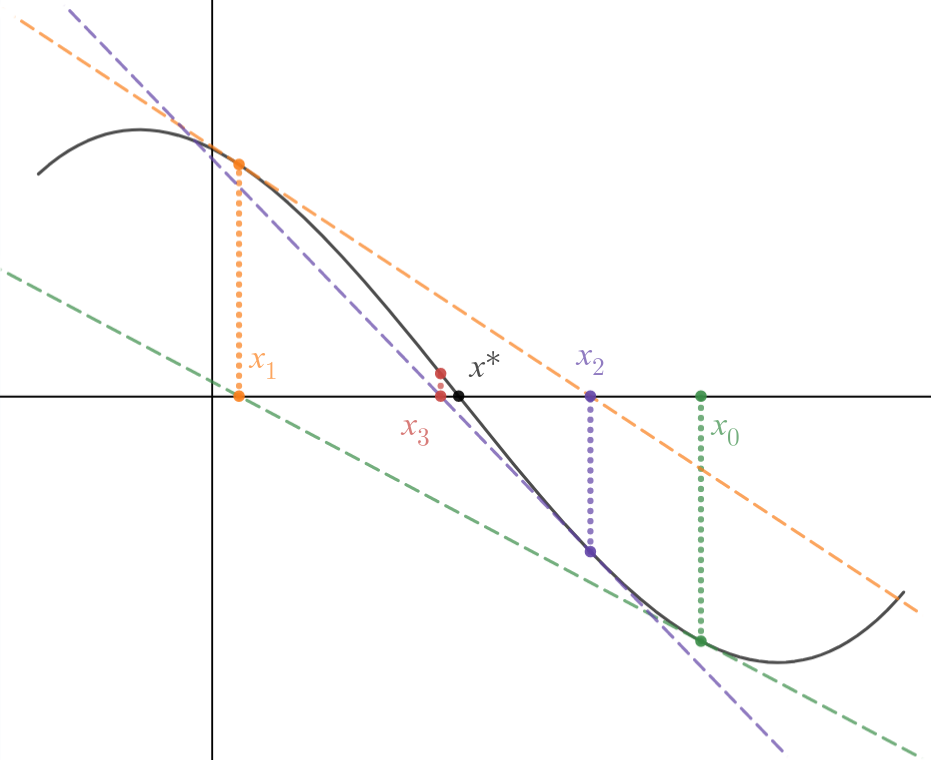
\includegraphics[width=10cm]{newton.png}
\caption{Interpretación geométrica del método de Newton.}
\label{fig:newton}
\end{figure}

Se trata de un método que, bajo las condiciones adecuadas, converge a una
buena velocidad. Sin embargo, tiene dos principales desventajas. Una de ellas
ya se mencionó anteriormente, y es la necesidad de conocer de antemano una
aproximación relativamente buena de la raíz buscada para poder asegurar la
convergencia; más aún si se desea que la convergencia sea rápida, ya que
el orden cuadrático puede resultar excesivamente lento si se comienza demasiado
lejos de la raíz. La otra desventaja es la necesidad de computar, en cada
paso, el valor de la derivada de $f$, lo cual puede ser difícil,
computacionalmente costoso o directamente imposible.

\subsection{Método de la secante}
El \textbf{método de la secante} es otra iteración de punto fijo que es
muy similar método de Newton, pero en lugar de considerar
la derivada de $f$ en el punto actual, la aproxima mediante la recta secante
que pasa por el punto actual y el punto anterior. Es decir, se considera que
\[ f'(x_k) \approx \frac{f(x_k) - f(x_{k-1})}{x_k - x_{k-1}}. \]

Como cada iteración tendrá en cuenta los dos puntos anteriores, se debe
comenzar determinando dos puntos iniciales, $x_0$ y $x_1$. Luego, la iteración
se define como
\[ x_{k+1} = x_k - \frac{f(x_k)}{\frac{f(x_k) - f(x_{k-1})}{x_k - x_{k-1}}}
           = x_k - \frac{f(x_k) \cdot (x_k - x_{k-1})}{f(x_k) - f(x_{k-1})}. \]

La Figura \ref{fig:secante} ilustra la interpretación geométrica de este
método.

\begin{figure}[H]
\centering
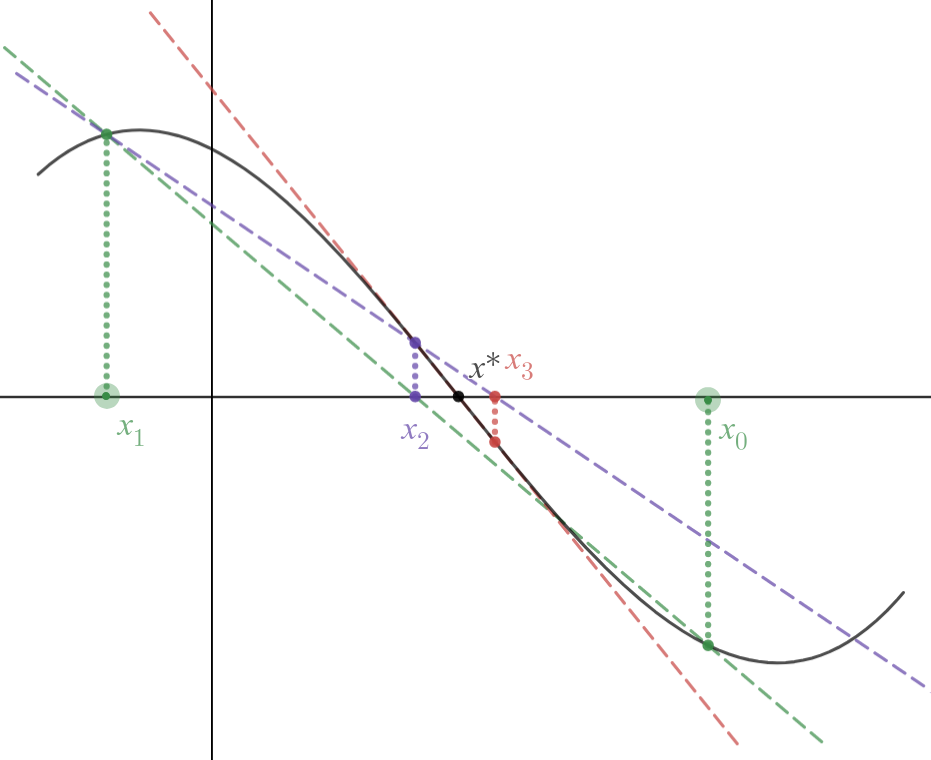
\includegraphics[width=10cm]{secante.png}
\caption{Interpretación geométrica del método de la secante.}
\label{fig:secante}
\end{figure}

El método de la secante converge un poco más lentamente que el método de
Newton. Sin embargo, puede demostrarse que su orden orden de convergencia es
supralineal: más exactamente, es $\varphi = \frac{1 + \sqrt{5}}{2}$, la
razón áurea. Además, presenta la gran ventaja de no requerir el cómputo
de ninguna derivada.

Uno de los inconvenientes que surge a la hora de utilizar este método tiene
que ver con la pérdida de dígitos significativos (o \emph{cancelación
catastrófica}) que se produce al tener que computar diferencias entre
valores que, con cada iteración, se encuentran cada vez más cerca; el método
\emph{regula falsi} presenta una alternativa que no padece de este problema.

\subsection{Método \emph{regula falsi}}
El \textbf{método \emph{regula falsi}} es una variante del método de
la bisección, que incorpora la idea principal del método de la secante.
Al igual que en el método de la bisección, se comienza con dos puntos
iniciales donde $f$ tiene distinto signo;
en cada paso se divide el intervalo en dos y se
pasa a trabajar con la parte en cuyos extremos $f$ tiene diferente signo.
Sin embargo, en lugar de dividir al intervalo por su punto medio, se utiliza
la intersección entre el eje de abscisas y la recta que pasa por los dos
puntos anteriores.

Este método converge con un orden lineal, de la misma forma que el método de
la bisección, pero resulta más rápido en términos prácticos. Comparado con
el método de la secante, si bien es más lento, reduce la posibilidad de que
se produzcan cancelaciones catastróficas: los valores de $f$ con los que
se trabaja siempre tienen signos opuestos, con lo cual las operaciones que se
realizan pueden pensarse como sumas en lugar de diferencias.


\end{document}
